\documentclass[10pt,a4paper]{article}
\usepackage[a4paper,left=1.8cm,right=1.8cm,top=1.6cm,bottom=2.0cm]{geometry}
\usepackage[T1]{fontenc}
\usepackage{helvet}
\renewcommand{\familydefault}{\sfdefault}
\usepackage[table]{xcolor}
\usepackage{graphicx,booktabs,array,float,caption,amsmath,enumitem,fancyhdr,titlesec,needspace}
\usepackage[hidelinks]{hyperref}

\definecolor{navy}{HTML}{1F3A5F}
\definecolor{zebra}{HTML}{F2F5F9}
\definecolor{hl}{HTML}{FFE9B3}
\definecolor{tagred}{HTML}{C0392B}
\definecolor{subtle}{HTML}{555555}

\setlength{\parindent}{0pt}
\setlength{\parskip}{5pt}
\setlength{\tabcolsep}{3pt}
\renewcommand{\arraystretch}{1.15}
\setlist{itemsep=2pt,topsep=2pt}
\captionsetup{font={small,color=subtle},labelfont=bf}
\titleformat{\section}{\Large\bfseries\color{navy}}{\thesection.}{0.5em}{}
\titleformat{\subsection}{\large\bfseries\color{navy}}{\thesubsection}{0.5em}{}

\pagestyle{fancy}
\fancyhf{}
\renewcommand{\headrulewidth}{0pt}
\fancyfoot[L]{\footnotesize\color{subtle}COMS4036A \textperiodcentered{} edit transferability \textperiodcentered{} results summary}
\fancyfoot[R]{\footnotesize\color{subtle}Page \thepage}

\hypersetup{pdftitle={Edit transferability: results summary},
            pdfauthor={Dylan Davies, Sudhir Adjodhya, Michael Badenhorst}}

\begin{document}
\begin{center}{\LARGE\bfseries Do edits that fool one face recognition model also fool models they were never built for?\par}\end{center}

\begin{center}\color{subtle}COMS4036A project \textperiodcentered{} results summary \textperiodcentered{} Dylan Davies, Sudhir Adjodhya, Michael Badenhorst\end{center}

\begin{center}\color{subtle}Generated from \emph{runs/sweep.csv}, \emph{runs/validate.csv}, \emph{runs/sweeps/} and \emph{runs/train.log}; every number below is read from those files.\end{center}

\needspace{8\baselineskip}\section{Summary}

We trained a face recognition network from scratch (the \textbf{surrogate}) and used projected gradient descent (PGD) against it to edit one photo in each of the 3,000 same-person pairs of the LFW View 2 benchmark. We then asked four models that were never used while editing whether they still recognise the pair as the same person.


\textbf{Main finding.} The edits work almost perfectly on the model they were built against and transfer poorly to everything else. At an edit budget of $\varepsilon$ = 4/255, where the edited photo is still nearly identical to the original (SSIM 0.955), the surrogate stops matching 100.0\% of same-person pairs, but the other deep models lose only 4.8\% (casia), 1.4\% (vggface2) and 0.4\% (arcface). Random noise at the same budget does almost nothing to any deep model, so the effect comes from the optimisation, not from changing pixels. Repeating the sweep with two more random seeds changes no result by more than 0.69 percentage points (standard deviation).


\textbf{Is it just our surrogate?} To check, we repeated the attack using each pretrained deep model as the attacker (Section 9). Our surrogate turns out to be the \emph{weakest} attacker of the four: at $\varepsilon$ = 8/255 its edits make casia lose 16.2\% of pairs, while edits built against vggface2 make casia lose 82.2\%. Edits transfer well \textbf{within the same architecture} (the three InceptionResnetV1 models) even when the training faces differ, while ArcFace, a different architecture, resists edits from every attacker (at most 18.8\%, even at a visible $\varepsilon$ = 16/255). So on the proposal's second question, the evidence points to \textbf{architecture} more than training data, and how well protection transfers depends heavily on which model the edit was built against.


\needspace{8\baselineskip}\section{Context: the question and why it matters}

Privacy tools such as Fawkes and LowKey add small, hard-to-see edits to photos before they are posted, so that face recognition systems can no longer link them to the person. These tools assume an edit built against one recognition system will also defeat whatever system someone else is running. A photo is edited once and must then hold up against every system that sees it later, so if edits do not \emph{transfer}, the protection is much weaker than it looks.


Our proposal asked two things: (1) when we edit a photo until \emph{our} model stops recognising it, do models we had no access to also stop recognising it? (2) Where some models resist and others give way, is that explained by their architecture or by the faces they were trained on? The four test models were chosen so that each differs from the surrogate in a controlled way.


\needspace{8\baselineskip}\section{Experimental setup}

\needspace{6\baselineskip}\subsection{Models}

\begin{center}\footnotesize
\begin{tabular}{>{\raggedright\arraybackslash}p{1.49cm}>{\raggedright\arraybackslash}p{2.99cm}>{\raggedright\arraybackslash}p{2.79cm}>{\raggedright\arraybackslash}p{2.59cm}>{\raggedright\arraybackslash}p{2.39cm}>{\raggedright\arraybackslash}p{3.19cm}}
\toprule
\rowcolor{navy}\textcolor{white}{\textbf{Model}} & \textcolor{white}{\textbf{Role}} & \textcolor{white}{\textbf{Architecture}} & \textcolor{white}{\textbf{Training faces}} & \textcolor{white}{\textbf{Training objective}} & \textcolor{white}{\textbf{Differs from surrogate in}} \\
\midrule
surrogate & Builds the edits (only model with gradients used) & InceptionResnetV1 & CASIA-WebFace (trained here) & Softmax cross-entropy & --- \\
\rowcolor{zebra}casia & Test model; also an attacker in Section 9 & InceptionResnetV1 & CASIA-WebFace & Softmax cross-entropy & Only the random initialisation \\
vggface2 & Test model; also an attacker in Section 9 & InceptionResnetV1 & VGGFace2 & Softmax cross-entropy & Training faces \\
\rowcolor{zebra}arcface & Test model; also an attacker in Section 9 & ResNet-50 (InsightFace buffalo\_l) & WebFace600K & ArcFace margin loss & Architecture, objective and faces \\
lbph & Test only & Local Binary Pattern Histograms & None (hand-crafted) & None & No deep learning at all \\
\bottomrule
\end{tabular}
\end{center}

\needspace{6\baselineskip}\subsection{Data}

\textbf{Test data:} LFW View 2, the standard benchmark of 6,000 fixed pairs (3,000 same-person, 3,000 different-person) split into 10 folds, covering 7,701 distinct photos. We use the published pairs unchanged, including the six known mislabelled pairs, as the maintainers request. The MTCNN face detector found a face in all 7,701 photos.


\textbf{Surrogate training data:} CASIA-WebFace, 490,623 images of 10,572 people, already aligned to 112$\times$112 pixels. LFW is too small to train on, so a separate dataset is needed; using CASIA means the surrogate shares its training faces with the casia test model, which is what lets us separate the effect of data from the effect of architecture.


\needspace{6\baselineskip}\subsection{How each model sees a photo}

Every edit is made on the full 250$\times$250 LFW photo, exactly as a user would post it. Each model then crops and aligns that same photo its own way, so every model sees the same edit:


\begin{itemize}
  \item  \textbf{vggface2 / casia:} a box crop around the detected face, 32-pixel margin, resized to 160$\times$160 (margin chosen by validation, Section 4).
  \item  \textbf{arcface / lbph:} the official InsightFace 5-point alignment to 112$\times$112 (eyes, nose, mouth corners).
  \item  \textbf{surrogate:} 5-point alignment to 160$\times$160, using landmark positions measured on the CASIA training crops, so its LFW test faces line up the way its training faces do.
\end{itemize}

All crops are implemented as one differentiable warp, so the surrogate's own cropping is part of the PGD optimisation. Face landmarks are detected once on the clean photo and reused for its edited versions.


\needspace{6\baselineskip}\subsection{Deciding ``same person''}

Each model turns a photo into an embedding and compares two photos by a distance (cosine distance for the deep models, chi-square for LBPH). A pair counts as the same person if the distance is below a threshold. Following the standard LFW protocol, each model gets its own threshold for each fold, fitted on the clean pairs of the other nine folds. These clean-data thresholds are then kept fixed when scoring edited photos, so a model's error rate at $\varepsilon$ = 0 is its ordinary baseline error.


\needspace{6\baselineskip}\subsection{The edit (PGD) and the comparisons}

PGD repeatedly nudges every pixel in the direction that makes the surrogate see the edited photo as \emph{more different from its own original}, then pulls any pixel that has moved further than $\varepsilon$ back within that limit. We push away from the photo's own original rather than from its pair partner because a real user does not know which photo their posted image will be compared against. Settings: $L_\infty$ budget $\varepsilon$, 20 steps, step size 2.5$\varepsilon$/20, random start. Edited photos are rounded back to ordinary 8-bit images before scoring.


\begin{center}\footnotesize
\begin{tabular}{>{\raggedright\arraybackslash}p{1.79cm}>{\raggedright\arraybackslash}p{4.09cm}>{\raggedright\arraybackslash}p{5.39cm}>{\raggedright\arraybackslash}p{4.59cm}}
\toprule
\rowcolor{navy}\textcolor{white}{\textbf{Condition}} & \textcolor{white}{\textbf{What it is}} & \textcolor{white}{\textbf{What it tells us}} & \textcolor{white}{\textbf{Strengths swept}} \\
\midrule
pgd & PGD edit against the surrogate & Main result & $\varepsilon$ = 0, 0.5, 1, 2, 4, 8, 16 (/255) \\
\rowcolor{zebra}noise & Random $\pm$$\varepsilon$ on every pixel & Whether the optimisation matters, or any change would do & Same $\varepsilon$ values \\
pgd+jpeg75 & PGD edit, then JPEG at quality 75 & Whether ordinary compression removes the edit & Same $\varepsilon$ values \\
\rowcolor{zebra}jpeg & JPEG compression of the clean photo & A free edit any user could apply & Quality 90, 75, 50, 30 \\
blur & Gaussian blur of the clean photo & A free edit any user could apply & $\sigma$ = 0.5, 1, 2, 3 pixels \\
\bottomrule
\end{tabular}
\end{center}

The \textbf{unmatched share} reported throughout is the fraction of the 3,000 same-person pairs that a model no longer accepts as the same person after photo \emph{a} of the pair is edited. Values are the mean over the 10 folds, $\pm$ the standard deviation across folds. \textbf{SSIM} (structural similarity, 1.0 = identical) measures how visible the edit is, comparing the edited photo with the original.


\needspace{8\baselineskip}\section{Validating the models before any edits}

The proposal identified alignment as the main risk: if a model is fed faces cropped the wrong way, it still produces numbers, just wrong ones. So before any edit we checked that each model reaches its published accuracy on clean LFW pairs. The gate was: every deep test model within about 1 percentage point of its published figure.


\begin{center}\footnotesize
\begin{tabular}{>{\raggedright\arraybackslash}p{2.19cm}>{\raggedright\arraybackslash}p{3.79cm}>{\raggedright\arraybackslash}p{2.79cm}>{\raggedright\arraybackslash}p{2.39cm}>{\raggedright\arraybackslash}p{2.19cm}}
\toprule
\rowcolor{navy}\textcolor{white}{\textbf{Model}} & \textcolor{white}{\textbf{Clean LFW accuracy (ours)}} & \textcolor{white}{\textbf{$\pm$ std over folds}} & \textcolor{white}{\textbf{Published}} & \textcolor{white}{\textbf{Gap}} \\
\midrule
surrogate & 98.12\% & 0.63\% & --- & --- \\
\rowcolor{zebra}casia & 98.73\% & 0.64\% & 99.05\% & -0.32 pts \\
vggface2 & 99.37\% & 0.33\% & 99.65\% & -0.28 pts \\
\rowcolor{zebra}arcface & 99.85\% & 0.17\% & 99.83\% & +0.02 pts \\
lbph & 67.03\% & 1.03\% & --- & --- \\
\bottomrule
\end{tabular}
\end{center}

All three pretrained deep models pass: ArcFace matches its published accuracy almost exactly, and the two facenet models sit about 0.3 points below theirs. The surrogate (trained by us) has no published figure; its accuracy is covered in Section 5. LBPH's 67\% is typical for a hand-crafted method on LFW and means it already gets many pairs wrong before any edit.


\textbf{Crop margin for the facenet models.} The facenet models are sensitive to how much border is kept around the face. We tried four margins and kept the best (32 pixels, which matches the original facenet LFW crop):


\begin{center}\footnotesize
\begin{tabular}{>{\raggedright\arraybackslash}p{2.99cm}>{\raggedright\arraybackslash}p{2.19cm}>{\raggedright\arraybackslash}p{2.19cm}>{\raggedright\arraybackslash}p{2.39cm}>{\raggedright\arraybackslash}p{2.19cm}}
\toprule
\rowcolor{navy}\textcolor{white}{\textbf{Margin (pixels)}} & \textcolor{white}{\textbf{0}} & \textcolor{white}{\textbf{14}} & \textcolor{white}{\textbf{32 (chosen)}} & \textcolor{white}{\textbf{44}} \\
\midrule
vggface2 & 99.00\% & 99.30\% & 99.37\% & 99.37\% \\
\rowcolor{zebra}casia & 98.07\% & 98.50\% & 98.73\% & 98.42\% \\
\bottomrule
\end{tabular}
\end{center}

\clearpage

\needspace{8\baselineskip}\section{Training the surrogate}

The surrogate is an InceptionResnetV1 trained from random initialisation for 30 epochs on CASIA-WebFace (1,916 steps of 256 images per epoch), using softmax cross-entropy over the 10,572 identities, SGD with Nesterov momentum 0.9, weight decay 5e-4, a one-cycle learning-rate schedule peaking at 0.1, bf16 mixed precision and random horizontal flips. Using the same architecture and objective as the facenet test models is deliberate, so that the casia model differs from the surrogate only in its random starting weights. Training took about 1.5 hours on an RTX 5070 Ti.


After each epoch the network was evaluated on clean LFW View 2 with the same 10-fold protocol. The saved model is the final epoch.


\begin{center}\footnotesize
\begin{tabular}{>{\raggedright\arraybackslash}p{1.39cm}>{\raggedright\arraybackslash}p{2.19cm}>{\raggedright\arraybackslash}p{2.59cm}>{\raggedright\arraybackslash}p{3.19cm}>{\raggedright\arraybackslash}p{1.79cm}}
\toprule
\rowcolor{navy}\textcolor{white}{\textbf{Epoch}} & \textcolor{white}{\textbf{Train loss}} & \textcolor{white}{\textbf{Train accuracy}} & \textcolor{white}{\textbf{Clean LFW accuracy}} & \textcolor{white}{\textbf{$\pm$ std}} \\
\midrule
1 & 7.875 & 3.7\% & 87.98\% & 1.57\% \\
\rowcolor{zebra}2 & 4.187 & 33.4\% & 92.63\% & 1.32\% \\
3 & 2.533 & 57.2\% & 94.47\% & 0.87\% \\
\rowcolor{zebra}4 & 2.069 & 65.6\% & 94.97\% & 0.99\% \\
5 & 1.853 & 69.8\% & 95.57\% & 0.81\% \\
\rowcolor{zebra}6 & 1.727 & 72.2\% & 95.77\% & 1.05\% \\
7 & 1.642 & 73.9\% & 96.27\% & 0.66\% \\
\rowcolor{zebra}8 & 1.581 & 75.1\% & 95.80\% & 0.62\% \\
9 & 1.529 & 76.1\% & 96.13\% & 1.09\% \\
\rowcolor{zebra}10 & 1.487 & 77.0\% & 96.58\% & 0.79\% \\
11 & 1.449 & 77.7\% & 97.27\% & 0.58\% \\
\rowcolor{zebra}12 & 1.411 & 78.5\% & 96.32\% & 0.88\% \\
13 & 1.375 & 79.2\% & 96.65\% & 0.93\% \\
\rowcolor{zebra}14 & 1.341 & 80.0\% & 97.18\% & 0.65\% \\
15 & 1.304 & 80.7\% & 97.30\% & 0.86\% \\
\rowcolor{zebra}16 & 1.261 & 81.6\% & 96.27\% & 0.99\% \\
17 & 1.218 & 82.4\% & 97.13\% & 0.85\% \\
\rowcolor{zebra}18 & 1.174 & 83.3\% & 97.68\% & 0.77\% \\
19 & 1.122 & 84.4\% & 97.65\% & 0.65\% \\
\rowcolor{zebra}20 & 1.067 & 85.4\% & 97.18\% & 0.75\% \\
21 & 1.007 & 86.5\% & 97.60\% & 0.64\% \\
\rowcolor{zebra}22 & 0.942 & 87.8\% & 97.88\% & 0.81\% \\
23 & 0.867 & 89.1\% & 97.90\% & 0.45\% \\
\rowcolor{zebra}24 & 0.782 & 90.6\% & 97.75\% & 0.57\% \\
25 & 0.689 & 92.0\% & 97.73\% & 0.55\% \\
\rowcolor{zebra}26 & 0.585 & 93.5\% & 98.00\% & 0.56\% \\
27 & 0.481 & 94.9\% & \cellcolor{hl}98.32\% & 0.49\% \\
\rowcolor{zebra}28 & 0.384 & 96.1\% & 98.17\% & 0.55\% \\
29 & 0.317 & 97.0\% & 98.20\% & 0.56\% \\
\rowcolor{zebra}30 & 0.285 & 97.4\% & 98.12\% & 0.63\% \\
\bottomrule
\end{tabular}
\end{center}

Clean LFW accuracy rose from 87.98\% after one epoch to 98.12\% after 30 (best 98.32\% in epoch 27, highlighted). For comparison, the published facenet model trained on the same data reaches 99.05\%, so the surrogate is a competent model, about one point weaker. Training accuracy reaching 97.4\% while LFW accuracy levels off means the last few epochs mostly fit the training set more tightly.


\clearpage

\needspace{8\baselineskip}\section{Main result: do PGD edits transfer?}

The table below is the core result of the project. Each cell is the share of the 3,000 same-person pairs the model no longer matches after one photo is edited with PGD against the surrogate. $\varepsilon$ = 0 means no edit, so that row is each model's baseline error. The SSIM column shows how visible the edit is at each budget.


\begin{center}\footnotesize
\begin{tabular}{>{\raggedright\arraybackslash}p{1.99cm}>{\raggedright\arraybackslash}p{2.49cm}>{\raggedright\arraybackslash}p{2.49cm}>{\raggedright\arraybackslash}p{2.49cm}>{\raggedright\arraybackslash}p{2.49cm}>{\raggedright\arraybackslash}p{2.49cm}>{\raggedright\arraybackslash}p{1.19cm}}
\toprule
\rowcolor{navy}\textcolor{white}{\textbf{Edit budget $\varepsilon$}} & \textcolor{white}{\textbf{surrogate}} & \textcolor{white}{\textbf{casia}} & \textcolor{white}{\textbf{vggface2}} & \textcolor{white}{\textbf{arcface}} & \textcolor{white}{\textbf{lbph}} & \textcolor{white}{\textbf{SSIM}} \\
\midrule
0/255 & 2.6\% $\pm$ 1.5\% & 1.8\% $\pm$ 1.4\% & 0.8\% $\pm$ 0.7\% & 0.3\% $\pm$ 0.4\% & 47.2\% $\pm$ 2.1\% & 1.000 \\
\rowcolor{zebra}0.5/255 & 6.1\% $\pm$ 2.1\% & 1.9\% $\pm$ 1.4\% & 0.8\% $\pm$ 0.7\% & 0.3\% $\pm$ 0.4\% & 45.4\% $\pm$ 1.8\% & 0.999 \\
1/255 & 20.6\% $\pm$ 4.5\% & 2.1\% $\pm$ 1.4\% & 0.8\% $\pm$ 0.7\% & 0.3\% $\pm$ 0.4\% & 42.8\% $\pm$ 1.9\% & 0.996 \\
\rowcolor{zebra}2/255 & 84.8\% $\pm$ 2.9\% & 2.6\% $\pm$ 1.7\% & 1.0\% $\pm$ 0.8\% & 0.3\% $\pm$ 0.4\% & 40.4\% $\pm$ 2.1\% & 0.987 \\
4/255 & 100.0\% $\pm$ 0.0\% & 4.8\% $\pm$ 2.0\% & 1.4\% $\pm$ 0.9\% & 0.4\% $\pm$ 0.5\% & 39.0\% $\pm$ 2.2\% & 0.955 \\
\rowcolor{zebra}8/255 & 100.0\% $\pm$ 0.0\% & 16.2\% $\pm$ 2.6\% & 3.3\% $\pm$ 1.6\% & 0.5\% $\pm$ 0.5\% & 44.5\% $\pm$ 2.8\% & 0.860 \\
16/255 & 100.0\% $\pm$ 0.0\% & 51.2\% $\pm$ 4.1\% & 12.0\% $\pm$ 2.6\% & 0.9\% $\pm$ 0.7\% & 65.4\% $\pm$ 2.1\% & 0.660 \\
\bottomrule
\end{tabular}
\end{center}

\begin{figure}[H]\centering
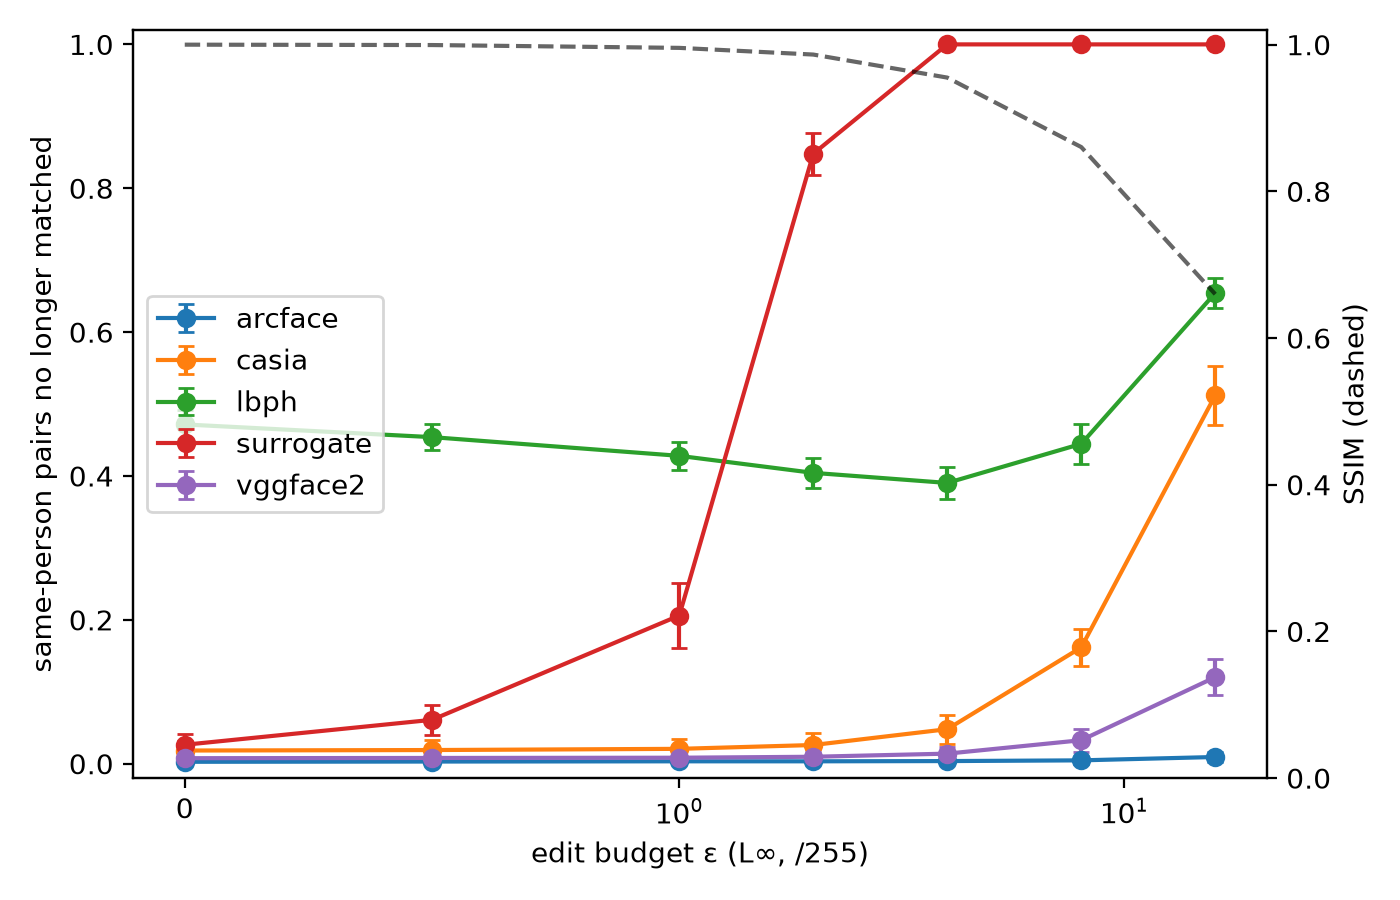
\includegraphics[width=15.5cm]{figures/main_result.png}
\caption{Share of same-person pairs no longer matched against edit budget (log scale), one line per model, error bars = std over 10 folds. Dashed line: SSIM between edited and original photo (right axis).}
\end{figure}

\needspace{6\baselineskip}\subsection{What the numbers say}

\textbf{The edit works on the model it was built against, and quickly.} The surrogate goes from a 2.6\% baseline to 20.6\% at $\varepsilon$ = 1/255, 84.8\% at 2/255 and 100.0\% from 4/255 upward. At 2/255 the edit is essentially invisible (SSIM 0.987).


\textbf{The edit barely transfers at invisible budgets.} At $\varepsilon$ = 4/255 (SSIM 0.955), every test deep model stays within a few points of its baseline: casia 1.8\% $\to$ 4.8\%, vggface2 0.8\% $\to$ 1.4\%, arcface 0.3\% $\to$ 0.4\%. A photo that is fully protected against the surrogate is still recognised by every other deep model about 95\% of the time or more.


\textbf{With our surrogate as attacker, shared training data looks decisive.} casia and vggface2 have the same architecture and objective; the only difference is that casia was trained on the same faces as the surrogate. At $\varepsilon$ = 16/255 casia loses 51.2\% of pairs while vggface2 loses 12.0\%, about four times less (at $\varepsilon$ = 8/255: 16.2\% vs 3.3\%). Changing architecture, objective and data together (arcface) removes transfer almost entirely: 0.9\% at $\varepsilon$ = 16/255. \emph{Section 9 shows this reading does not hold once other models are used as the attacker.}


\textbf{Visible edits are needed before anything transfers.} The only substantial transfer (casia, 51.2\%) happens at $\varepsilon$ = 16/255, where SSIM has dropped to 0.660 and the edit is clearly visible. So in our setting, an edit that is invisible is not transferable, and an edit that transfers is not invisible.


\clearpage

\needspace{8\baselineskip}\section{Required comparisons}

\needspace{6\baselineskip}\subsection{Random noise at the same budget}

Random noise changes every pixel by exactly $\pm$$\varepsilon$, the same maximum change PGD is allowed. If noise did as well as PGD, the optimisation would be contributing nothing.


\begin{center}\footnotesize
\begin{tabular}{>{\raggedright\arraybackslash}p{1.99cm}>{\raggedright\arraybackslash}p{2.49cm}>{\raggedright\arraybackslash}p{2.49cm}>{\raggedright\arraybackslash}p{2.49cm}>{\raggedright\arraybackslash}p{2.49cm}>{\raggedright\arraybackslash}p{2.49cm}>{\raggedright\arraybackslash}p{1.19cm}}
\toprule
\rowcolor{navy}\textcolor{white}{\textbf{Noise budget $\varepsilon$}} & \textcolor{white}{\textbf{surrogate}} & \textcolor{white}{\textbf{casia}} & \textcolor{white}{\textbf{vggface2}} & \textcolor{white}{\textbf{arcface}} & \textcolor{white}{\textbf{lbph}} & \textcolor{white}{\textbf{SSIM}} \\
\midrule
0/255 & 2.6\% $\pm$ 1.5\% & 1.8\% $\pm$ 1.4\% & 0.8\% $\pm$ 0.7\% & 0.3\% $\pm$ 0.4\% & 47.2\% $\pm$ 2.1\% & 1.000 \\
\rowcolor{zebra}0.5/255 & 2.6\% $\pm$ 1.6\% & 1.8\% $\pm$ 1.4\% & 0.8\% $\pm$ 0.7\% & 0.3\% $\pm$ 0.4\% & 45.2\% $\pm$ 2.1\% & 0.997 \\
1/255 & 2.5\% $\pm$ 1.4\% & 1.9\% $\pm$ 1.4\% & 0.8\% $\pm$ 0.7\% & 0.3\% $\pm$ 0.4\% & 43.7\% $\pm$ 2.1\% & 0.992 \\
\rowcolor{zebra}2/255 & 2.7\% $\pm$ 1.5\% & 1.8\% $\pm$ 1.4\% & 0.8\% $\pm$ 0.8\% & 0.3\% $\pm$ 0.4\% & 42.4\% $\pm$ 2.0\% & 0.969 \\
4/255 & 2.9\% $\pm$ 1.7\% & 2.0\% $\pm$ 1.4\% & 0.8\% $\pm$ 0.8\% & 0.3\% $\pm$ 0.4\% & 47.3\% $\pm$ 2.3\% & 0.893 \\
\rowcolor{zebra}8/255 & 3.6\% $\pm$ 2.0\% & 2.4\% $\pm$ 1.4\% & 0.9\% $\pm$ 0.7\% & 0.3\% $\pm$ 0.4\% & 65.4\% $\pm$ 2.6\% & 0.713 \\
16/255 & 7.4\% $\pm$ 2.4\% & 4.3\% $\pm$ 1.6\% & 1.4\% $\pm$ 0.6\% & 0.4\% $\pm$ 0.5\% & 90.1\% $\pm$ 2.0\% & 0.462 \\
\bottomrule
\end{tabular}
\end{center}

Noise does almost nothing to any deep model. Even at $\varepsilon$ = 16/255, where noise is more visible than PGD (SSIM 0.462 vs 0.660), the surrogate only reaches 7.4\% against 100.0\% for PGD, and casia 4.3\% against 51.2\%. The PGD effect, and the transfer to casia, therefore come from the optimisation itself.


\needspace{6\baselineskip}\subsection{JPEG compression after editing}

Photos are usually recompressed when uploaded. Here the PGD-edited photo is saved as JPEG at quality 75 before the models see it. The SSIM column includes the compression's own loss of detail.


\begin{center}\footnotesize
\begin{tabular}{>{\raggedright\arraybackslash}p{1.99cm}>{\raggedright\arraybackslash}p{2.49cm}>{\raggedright\arraybackslash}p{2.49cm}>{\raggedright\arraybackslash}p{2.49cm}>{\raggedright\arraybackslash}p{2.49cm}>{\raggedright\arraybackslash}p{2.49cm}>{\raggedright\arraybackslash}p{1.19cm}}
\toprule
\rowcolor{navy}\textcolor{white}{\textbf{Edit budget $\varepsilon$}} & \textcolor{white}{\textbf{surrogate}} & \textcolor{white}{\textbf{casia}} & \textcolor{white}{\textbf{vggface2}} & \textcolor{white}{\textbf{arcface}} & \textcolor{white}{\textbf{lbph}} & \textcolor{white}{\textbf{SSIM}} \\
\midrule
0/255 & 2.6\% $\pm$ 1.8\% & 1.9\% $\pm$ 1.4\% & 0.8\% $\pm$ 0.7\% & 0.3\% $\pm$ 0.4\% & 48.3\% $\pm$ 2.2\% & 0.973 \\
\rowcolor{zebra}0.5/255 & 4.0\% $\pm$ 1.9\% & 2.1\% $\pm$ 1.4\% & 0.8\% $\pm$ 0.7\% & 0.3\% $\pm$ 0.4\% & 45.6\% $\pm$ 1.4\% & 0.973 \\
1/255 & 8.2\% $\pm$ 4.0\% & 2.1\% $\pm$ 1.4\% & 0.9\% $\pm$ 0.8\% & 0.3\% $\pm$ 0.4\% & 42.7\% $\pm$ 1.7\% & 0.972 \\
\rowcolor{zebra}2/255 & 39.1\% $\pm$ 6.3\% & 2.7\% $\pm$ 1.5\% & 0.9\% $\pm$ 0.8\% & 0.3\% $\pm$ 0.4\% & 39.6\% $\pm$ 1.8\% & 0.968 \\
4/255 & 97.1\% $\pm$ 1.0\% & 4.5\% $\pm$ 1.7\% & 1.3\% $\pm$ 0.9\% & 0.4\% $\pm$ 0.5\% & 36.5\% $\pm$ 1.9\% & 0.960 \\
\rowcolor{zebra}8/255 & 100.0\% $\pm$ 0.0\% & 12.3\% $\pm$ 2.8\% & 2.9\% $\pm$ 1.5\% & 0.5\% $\pm$ 0.5\% & 35.7\% $\pm$ 2.2\% & 0.928 \\
16/255 & 100.0\% $\pm$ 0.0\% & 43.2\% $\pm$ 4.0\% & 10.1\% $\pm$ 2.0\% & 0.8\% $\pm$ 0.7\% & 48.5\% $\pm$ 2.5\% & 0.820 \\
\bottomrule
\end{tabular}
\end{center}

Compression weakens small edits but does not remove larger ones. Against the surrogate, at $\varepsilon$ = 2/255 it cuts the unmatched share from 84.8\% to 39.1\%; at $\varepsilon$ = 4/255 the edit survives (97.1\%) and from 8/255 it is unaffected. Transfer to casia at $\varepsilon$ = 16/255 drops slightly, from 51.2\% to 43.2\%.


\begin{figure}[H]\centering
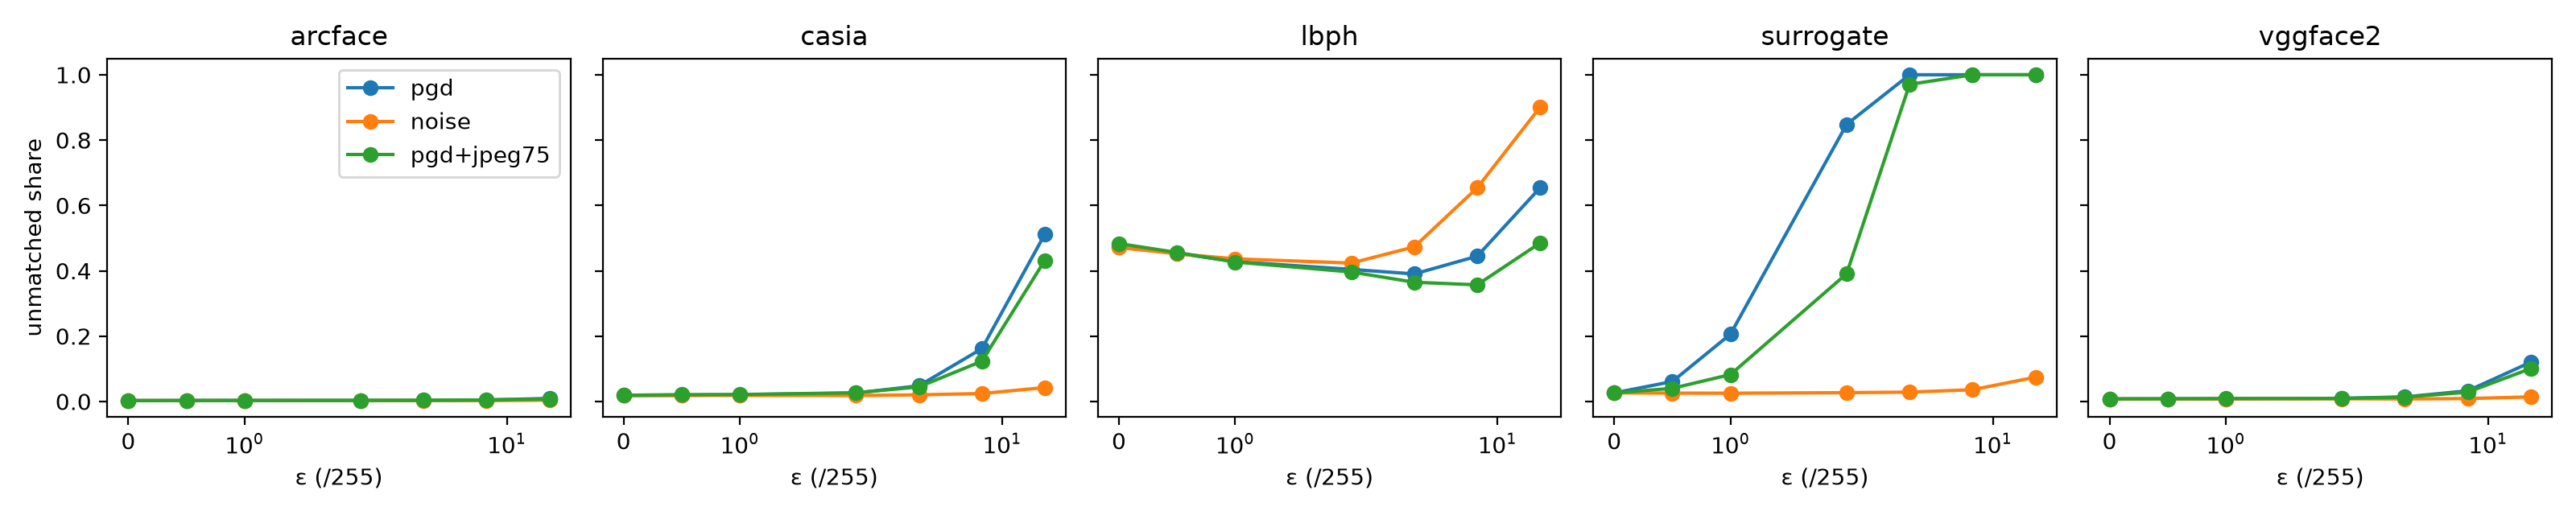
\includegraphics[width=17.0cm]{figures/edit_comparison.png}
\caption{PGD vs random noise vs PGD followed by JPEG (quality 75), one panel per model (unmatched share vs $\varepsilon$).}
\end{figure}

\clearpage

\needspace{6\baselineskip}\subsection{Free edits: JPEG compression and blur of the original photo}

These are things any user could do without special tools. They are applied to the clean photo, with no PGD.


\begin{center}\footnotesize
\begin{tabular}{>{\raggedright\arraybackslash}p{1.99cm}>{\raggedright\arraybackslash}p{2.49cm}>{\raggedright\arraybackslash}p{2.49cm}>{\raggedright\arraybackslash}p{2.49cm}>{\raggedright\arraybackslash}p{2.49cm}>{\raggedright\arraybackslash}p{2.49cm}>{\raggedright\arraybackslash}p{1.19cm}}
\toprule
\rowcolor{navy}\textcolor{white}{\textbf{JPEG quality}} & \textcolor{white}{\textbf{surrogate}} & \textcolor{white}{\textbf{casia}} & \textcolor{white}{\textbf{vggface2}} & \textcolor{white}{\textbf{arcface}} & \textcolor{white}{\textbf{lbph}} & \textcolor{white}{\textbf{SSIM}} \\
\midrule
30 & 3.4\% $\pm$ 1.9\% & 2.0\% $\pm$ 1.3\% & 0.8\% $\pm$ 0.8\% & 0.3\% $\pm$ 0.4\% & 54.9\% $\pm$ 2.5\% & 0.927 \\
\rowcolor{zebra}50 & 2.8\% $\pm$ 1.6\% & 1.9\% $\pm$ 1.4\% & 0.8\% $\pm$ 0.8\% & 0.3\% $\pm$ 0.4\% & 49.2\% $\pm$ 2.0\% & 0.952 \\
75 & 2.6\% $\pm$ 1.8\% & 1.9\% $\pm$ 1.4\% & 0.8\% $\pm$ 0.7\% & 0.3\% $\pm$ 0.4\% & 48.3\% $\pm$ 2.2\% & 0.973 \\
\rowcolor{zebra}90 & 2.6\% $\pm$ 1.5\% & 1.8\% $\pm$ 1.4\% & 0.8\% $\pm$ 0.7\% & 0.3\% $\pm$ 0.4\% & 47.2\% $\pm$ 2.2\% & 0.999 \\
\bottomrule
\end{tabular}
\end{center}

\begin{center}\footnotesize
\begin{tabular}{>{\raggedright\arraybackslash}p{1.99cm}>{\raggedright\arraybackslash}p{2.49cm}>{\raggedright\arraybackslash}p{2.49cm}>{\raggedright\arraybackslash}p{2.49cm}>{\raggedright\arraybackslash}p{2.49cm}>{\raggedright\arraybackslash}p{2.49cm}>{\raggedright\arraybackslash}p{1.19cm}}
\toprule
\rowcolor{navy}\textcolor{white}{\textbf{Blur $\sigma$ (px)}} & \textcolor{white}{\textbf{surrogate}} & \textcolor{white}{\textbf{casia}} & \textcolor{white}{\textbf{vggface2}} & \textcolor{white}{\textbf{arcface}} & \textcolor{white}{\textbf{lbph}} & \textcolor{white}{\textbf{SSIM}} \\
\midrule
0.5 & 2.5\% $\pm$ 1.5\% & 1.8\% $\pm$ 1.4\% & 0.8\% $\pm$ 0.8\% & 0.3\% $\pm$ 0.4\% & 52.6\% $\pm$ 3.0\% & 0.996 \\
\rowcolor{zebra}1 & 2.9\% $\pm$ 1.9\% & 2.1\% $\pm$ 1.2\% & 0.9\% $\pm$ 0.7\% & 0.3\% $\pm$ 0.4\% & 77.2\% $\pm$ 2.2\% & 0.965 \\
2 & 7.9\% $\pm$ 2.9\% & 5.2\% $\pm$ 1.6\% & 2.1\% $\pm$ 1.1\% & 0.3\% $\pm$ 0.4\% & 97.4\% $\pm$ 0.7\% & 0.876 \\
\rowcolor{zebra}3 & 22.2\% $\pm$ 5.5\% & 16.6\% $\pm$ 2.6\% & 6.8\% $\pm$ 2.1\% & 0.7\% $\pm$ 0.5\% & 99.6\% $\pm$ 0.2\% & 0.790 \\
\bottomrule
\end{tabular}
\end{center}

JPEG compression, even at quality 30, leaves the deep models essentially unaffected (surrogate 3.4\%, casia 2.0\%). Blur starts to matter only when strong: at $\sigma$ = 3 pixels (SSIM 0.790) the surrogate loses 22.2\% and casia 16.6\%, while arcface stays at 0.7\%. Free edits are not a substitute for an optimised edit.


\begin{figure}[H]\centering
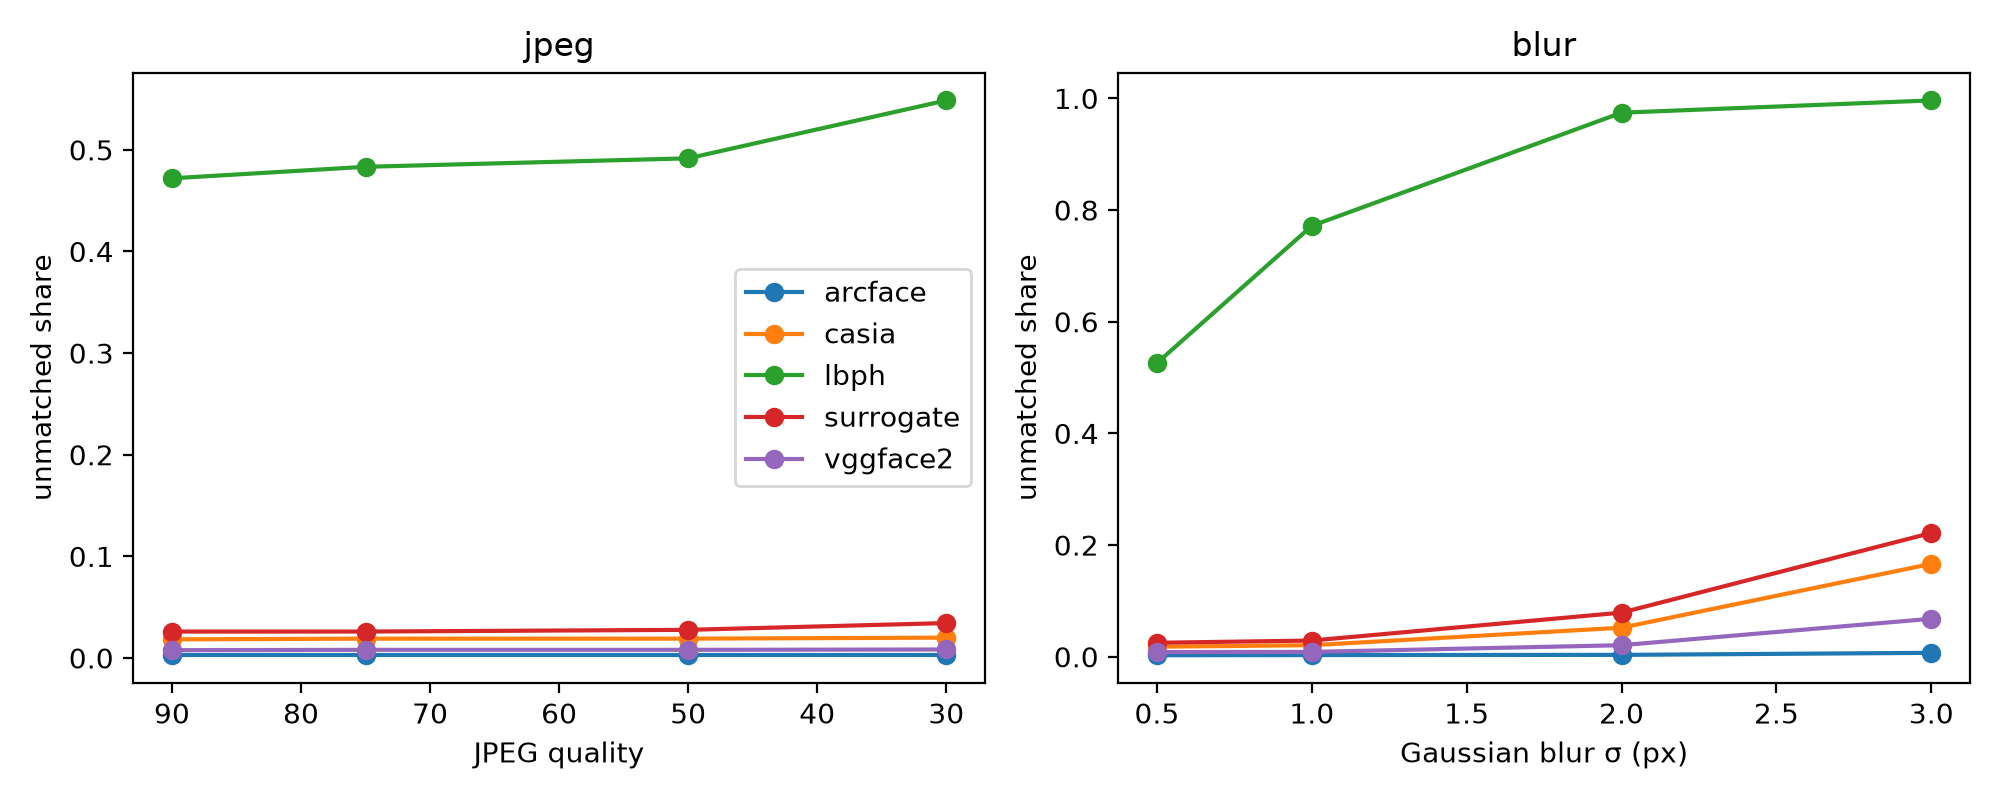
\includegraphics[width=16.0cm]{figures/free_edits.png}
\caption{Unmatched share under JPEG compression (left, quality decreasing to the right) and Gaussian blur (right).}
\end{figure}

\clearpage

\needspace{8\baselineskip}\section{Are the results stable? Two more random seeds}

The seed controls PGD's random starting point and the random-noise baseline, so re-running with different seeds shows how much of the result is luck. We repeated the full surrogate sweep (all conditions, all 3,000 pairs) with seeds 1 and 2, in addition to the original seed 0. The table shows, for PGD, the unmatched share averaged over the 10 folds for each seed, then the mean $\pm$ standard deviation across the three seeds (std in percentage points).


\begin{center}\footnotesize
\begin{tabular}{>{\raggedright\arraybackslash}p{2.19cm}>{\raggedright\arraybackslash}p{2.79cm}>{\raggedright\arraybackslash}p{2.79cm}>{\raggedright\arraybackslash}p{2.79cm}>{\raggedright\arraybackslash}p{2.79cm}>{\raggedright\arraybackslash}p{2.79cm}}
\toprule
\rowcolor{navy}\textcolor{white}{\textbf{Edit budget $\varepsilon$}} & \textcolor{white}{\textbf{surrogate}} & \textcolor{white}{\textbf{casia}} & \textcolor{white}{\textbf{vggface2}} & \textcolor{white}{\textbf{arcface}} & \textcolor{white}{\textbf{lbph}} \\
\midrule
0/255 & 2.63\% $\pm$ 0.00 & 1.83\% $\pm$ 0.00 & 0.77\% $\pm$ 0.00 & 0.27\% $\pm$ 0.00 & 47.17\% $\pm$ 0.00 \\
\rowcolor{zebra}0.5/255 & 5.98\% $\pm$ 0.13 & 1.90\% $\pm$ 0.07 & 0.77\% $\pm$ 0.03 & 0.29\% $\pm$ 0.02 & 45.32\% $\pm$ 0.11 \\
1/255 & 20.34\% $\pm$ 0.36 & 2.10\% $\pm$ 0.06 & 0.78\% $\pm$ 0.07 & 0.32\% $\pm$ 0.02 & 43.10\% $\pm$ 0.27 \\
\rowcolor{zebra}2/255 & 84.08\% $\pm$ 0.69 & 2.72\% $\pm$ 0.12 & 0.93\% $\pm$ 0.06 & 0.36\% $\pm$ 0.02 & 40.63\% $\pm$ 0.18 \\
4/255 & 100.00\% $\pm$ 0.00 & 4.94\% $\pm$ 0.13 & 1.44\% $\pm$ 0.05 & 0.40\% $\pm$ 0.03 & 39.06\% $\pm$ 0.23 \\
\rowcolor{zebra}8/255 & 100.00\% $\pm$ 0.00 & 15.90\% $\pm$ 0.23 & 3.29\% $\pm$ 0.13 & 0.49\% $\pm$ 0.04 & 44.44\% $\pm$ 0.13 \\
16/255 & 100.00\% $\pm$ 0.00 & 50.93\% $\pm$ 0.38 & 11.70\% $\pm$ 0.31 & 1.06\% $\pm$ 0.13 & 65.18\% $\pm$ 0.29 \\
\bottomrule
\end{tabular}
\end{center}

Largest standard deviation across seeds for each condition: blur 0.00 pts, jpeg 0.00 pts, noise 0.33 pts, pgd 0.69 pts, pgd+jpeg75 0.55 pts. JPEG and blur involve no randomness, so they are identical across seeds. Every result in this document is reproducible to well under one percentage point; the differences between models are far larger than seed noise.


\needspace{8\baselineskip}\section{Is it just our surrogate? Every deep model as the attacker}

A worry with Section 6 is that our surrogate might simply be a poor model to build edits against, for example because it overfits its training data. To test this, we ran the same PGD attack using each of the other deep models as the attacker (casia, vggface2 and arcface, all at seed 0) and scored the edited photos on all five models. LBPH cannot be an attacker because it has no gradients. ArcFace was converted from its ONNX file to PyTorch (onnx2torch) so gradients could flow through it; the converted model gives the same clean LFW accuracy (99.85\%).


Each table below gives the share of same-person pairs the \textbf{target} (column) stops matching when the edit was built against the \textbf{attacker} (row), mean $\pm$ std over the 10 folds. Highlighted cells are each attacker against itself. The SSIM column shows the edits are equally visible whichever model built them.


\par\noindent\begin{minipage}{\linewidth}
\par\smallskip\noindent\textbf{$\varepsilon$ = 2/255 (essentially invisible)}\par\smallskip
\begin{center}\footnotesize
\begin{tabular}{>{\raggedright\arraybackslash}p{2.89cm}>{\raggedright\arraybackslash}p{2.29cm}>{\raggedright\arraybackslash}p{2.29cm}>{\raggedright\arraybackslash}p{2.29cm}>{\raggedright\arraybackslash}p{2.29cm}>{\raggedright\arraybackslash}p{2.29cm}>{\raggedright\arraybackslash}p{1.09cm}}
\toprule
\rowcolor{navy}\textcolor{white}{\textbf{Attacker $\downarrow$ \textperiodcentered{} target $\to$}} & \textcolor{white}{\textbf{surrogate}} & \textcolor{white}{\textbf{casia}} & \textcolor{white}{\textbf{vggface2}} & \textcolor{white}{\textbf{arcface}} & \textcolor{white}{\textbf{lbph}} & \textcolor{white}{\textbf{SSIM}} \\
\midrule
surrogate & \cellcolor{hl}84.8\% $\pm$ 2.9\% & 2.6\% $\pm$ 1.7\% & 1.0\% $\pm$ 0.8\% & 0.3\% $\pm$ 0.4\% & 40.4\% $\pm$ 2.1\% & 0.987 \\
\rowcolor{zebra}casia & 6.1\% $\pm$ 2.6\% & \cellcolor{hl}38.8\% $\pm$ 3.9\% & 1.5\% $\pm$ 0.9\% & 0.3\% $\pm$ 0.4\% & 41.5\% $\pm$ 2.0\% & 0.986 \\
vggface2 & 5.6\% $\pm$ 3.1\% & 3.8\% $\pm$ 1.6\% & \cellcolor{hl}27.2\% $\pm$ 4.1\% & 0.4\% $\pm$ 0.5\% & 41.8\% $\pm$ 2.0\% & 0.986 \\
\rowcolor{zebra}arcface & 4.0\% $\pm$ 2.3\% & 2.8\% $\pm$ 1.3\% & 1.1\% $\pm$ 0.7\% & \cellcolor{hl}11.2\% $\pm$ 2.2\% & 42.1\% $\pm$ 1.8\% & 0.986 \\
\bottomrule
\end{tabular}
\end{center}
\end{minipage}\par\medskip

\par\noindent\begin{minipage}{\linewidth}
\par\smallskip\noindent\textbf{$\varepsilon$ = 4/255 (nearly invisible)}\par\smallskip
\begin{center}\footnotesize
\begin{tabular}{>{\raggedright\arraybackslash}p{2.89cm}>{\raggedright\arraybackslash}p{2.29cm}>{\raggedright\arraybackslash}p{2.29cm}>{\raggedright\arraybackslash}p{2.29cm}>{\raggedright\arraybackslash}p{2.29cm}>{\raggedright\arraybackslash}p{2.29cm}>{\raggedright\arraybackslash}p{1.09cm}}
\toprule
\rowcolor{navy}\textcolor{white}{\textbf{Attacker $\downarrow$ \textperiodcentered{} target $\to$}} & \textcolor{white}{\textbf{surrogate}} & \textcolor{white}{\textbf{casia}} & \textcolor{white}{\textbf{vggface2}} & \textcolor{white}{\textbf{arcface}} & \textcolor{white}{\textbf{lbph}} & \textcolor{white}{\textbf{SSIM}} \\
\midrule
surrogate & \cellcolor{hl}100.0\% $\pm$ 0.0\% & 4.8\% $\pm$ 2.0\% & 1.4\% $\pm$ 0.9\% & 0.4\% $\pm$ 0.5\% & 39.0\% $\pm$ 2.2\% & 0.955 \\
\rowcolor{zebra}casia & 30.9\% $\pm$ 4.6\% & \cellcolor{hl}98.9\% $\pm$ 0.6\% & 6.4\% $\pm$ 1.8\% & 0.4\% $\pm$ 0.5\% & 40.3\% $\pm$ 2.1\% & 0.953 \\
vggface2 & 23.1\% $\pm$ 5.2\% & 22.7\% $\pm$ 3.2\% & \cellcolor{hl}95.3\% $\pm$ 1.5\% & 0.5\% $\pm$ 0.4\% & 40.1\% $\pm$ 2.1\% & 0.954 \\
\rowcolor{zebra}arcface & 9.9\% $\pm$ 3.4\% & 5.5\% $\pm$ 1.3\% & 2.1\% $\pm$ 1.4\% & \cellcolor{hl}95.9\% $\pm$ 1.5\% & 41.5\% $\pm$ 2.1\% & 0.953 \\
\bottomrule
\end{tabular}
\end{center}
\end{minipage}\par\medskip

\par\noindent\begin{minipage}{\linewidth}
\par\smallskip\noindent\textbf{$\varepsilon$ = 8/255}\par\smallskip
\begin{center}\footnotesize
\begin{tabular}{>{\raggedright\arraybackslash}p{2.89cm}>{\raggedright\arraybackslash}p{2.29cm}>{\raggedright\arraybackslash}p{2.29cm}>{\raggedright\arraybackslash}p{2.29cm}>{\raggedright\arraybackslash}p{2.29cm}>{\raggedright\arraybackslash}p{2.29cm}>{\raggedright\arraybackslash}p{1.09cm}}
\toprule
\rowcolor{navy}\textcolor{white}{\textbf{Attacker $\downarrow$ \textperiodcentered{} target $\to$}} & \textcolor{white}{\textbf{surrogate}} & \textcolor{white}{\textbf{casia}} & \textcolor{white}{\textbf{vggface2}} & \textcolor{white}{\textbf{arcface}} & \textcolor{white}{\textbf{lbph}} & \textcolor{white}{\textbf{SSIM}} \\
\midrule
surrogate & \cellcolor{hl}100.0\% $\pm$ 0.0\% & 16.2\% $\pm$ 2.6\% & 3.3\% $\pm$ 1.6\% & 0.5\% $\pm$ 0.5\% & 44.5\% $\pm$ 2.8\% & 0.860 \\
\rowcolor{zebra}casia & 84.3\% $\pm$ 4.0\% & \cellcolor{hl}100.0\% $\pm$ 0.0\% & 32.0\% $\pm$ 4.4\% & 1.3\% $\pm$ 0.7\% & 45.6\% $\pm$ 2.5\% & 0.856 \\
vggface2 & 76.5\% $\pm$ 4.2\% & 82.2\% $\pm$ 3.2\% & \cellcolor{hl}100.0\% $\pm$ 0.0\% & 3.7\% $\pm$ 1.2\% & 42.6\% $\pm$ 2.2\% & 0.857 \\
\rowcolor{zebra}arcface & 29.6\% $\pm$ 5.1\% & 16.2\% $\pm$ 2.6\% & 6.2\% $\pm$ 2.5\% & \cellcolor{hl}100.0\% $\pm$ 0.0\% & 46.4\% $\pm$ 2.6\% & 0.856 \\
\bottomrule
\end{tabular}
\end{center}
\end{minipage}\par\medskip

\par\noindent\begin{minipage}{\linewidth}
\par\smallskip\noindent\textbf{$\varepsilon$ = 16/255 (clearly visible)}\par\smallskip
\begin{center}\footnotesize
\begin{tabular}{>{\raggedright\arraybackslash}p{2.89cm}>{\raggedright\arraybackslash}p{2.29cm}>{\raggedright\arraybackslash}p{2.29cm}>{\raggedright\arraybackslash}p{2.29cm}>{\raggedright\arraybackslash}p{2.29cm}>{\raggedright\arraybackslash}p{2.29cm}>{\raggedright\arraybackslash}p{1.09cm}}
\toprule
\rowcolor{navy}\textcolor{white}{\textbf{Attacker $\downarrow$ \textperiodcentered{} target $\to$}} & \textcolor{white}{\textbf{surrogate}} & \textcolor{white}{\textbf{casia}} & \textcolor{white}{\textbf{vggface2}} & \textcolor{white}{\textbf{arcface}} & \textcolor{white}{\textbf{lbph}} & \textcolor{white}{\textbf{SSIM}} \\
\midrule
surrogate & \cellcolor{hl}100.0\% $\pm$ 0.0\% & 51.2\% $\pm$ 4.1\% & 12.0\% $\pm$ 2.6\% & 0.9\% $\pm$ 0.7\% & 65.4\% $\pm$ 2.1\% & 0.660 \\
\rowcolor{zebra}casia & 97.9\% $\pm$ 1.0\% & \cellcolor{hl}100.0\% $\pm$ 0.0\% & 75.5\% $\pm$ 1.8\% & 7.3\% $\pm$ 1.3\% & 65.5\% $\pm$ 2.6\% & 0.656 \\
vggface2 & 97.3\% $\pm$ 1.1\% & 98.7\% $\pm$ 1.0\% & \cellcolor{hl}100.0\% $\pm$ 0.0\% & 18.8\% $\pm$ 3.3\% & 60.1\% $\pm$ 2.7\% & 0.657 \\
\rowcolor{zebra}arcface & 61.9\% $\pm$ 6.4\% & 45.9\% $\pm$ 4.1\% & 21.4\% $\pm$ 3.8\% & \cellcolor{hl}100.0\% $\pm$ 0.0\% & 65.5\% $\pm$ 2.3\% & 0.655 \\
\bottomrule
\end{tabular}
\end{center}
\end{minipage}\par\medskip

\par\noindent\begin{minipage}{\linewidth}
\par\smallskip\noindent\textbf{$\varepsilon$ = 8/255, edit then JPEG quality 75}\par\smallskip
\begin{center}\footnotesize
\begin{tabular}{>{\raggedright\arraybackslash}p{2.89cm}>{\raggedright\arraybackslash}p{2.29cm}>{\raggedright\arraybackslash}p{2.29cm}>{\raggedright\arraybackslash}p{2.29cm}>{\raggedright\arraybackslash}p{2.29cm}>{\raggedright\arraybackslash}p{2.29cm}>{\raggedright\arraybackslash}p{1.09cm}}
\toprule
\rowcolor{navy}\textcolor{white}{\textbf{Attacker $\downarrow$ \textperiodcentered{} target $\to$}} & \textcolor{white}{\textbf{surrogate}} & \textcolor{white}{\textbf{casia}} & \textcolor{white}{\textbf{vggface2}} & \textcolor{white}{\textbf{arcface}} & \textcolor{white}{\textbf{lbph}} & \textcolor{white}{\textbf{SSIM}} \\
\midrule
surrogate & \cellcolor{hl}100.0\% $\pm$ 0.0\% & 12.3\% $\pm$ 2.8\% & 2.9\% $\pm$ 1.5\% & 0.5\% $\pm$ 0.5\% & 35.7\% $\pm$ 2.2\% & 0.928 \\
\rowcolor{zebra}casia & 76.8\% $\pm$ 5.1\% & \cellcolor{hl}100.0\% $\pm$ 0.0\% & 23.3\% $\pm$ 3.1\% & 0.9\% $\pm$ 0.9\% & 38.7\% $\pm$ 1.9\% & 0.923 \\
vggface2 & 71.8\% $\pm$ 4.6\% & 74.7\% $\pm$ 3.3\% & \cellcolor{hl}100.0\% $\pm$ 0.0\% & 2.3\% $\pm$ 0.9\% & 36.1\% $\pm$ 2.0\% & 0.923 \\
\rowcolor{zebra}arcface & 25.0\% $\pm$ 4.6\% & 13.7\% $\pm$ 2.4\% & 5.3\% $\pm$ 2.0\% & \cellcolor{hl}99.9\% $\pm$ 0.1\% & 37.0\% $\pm$ 2.4\% & 0.923 \\
\bottomrule
\end{tabular}
\end{center}
\end{minipage}\par\medskip

\begin{figure}[H]\centering
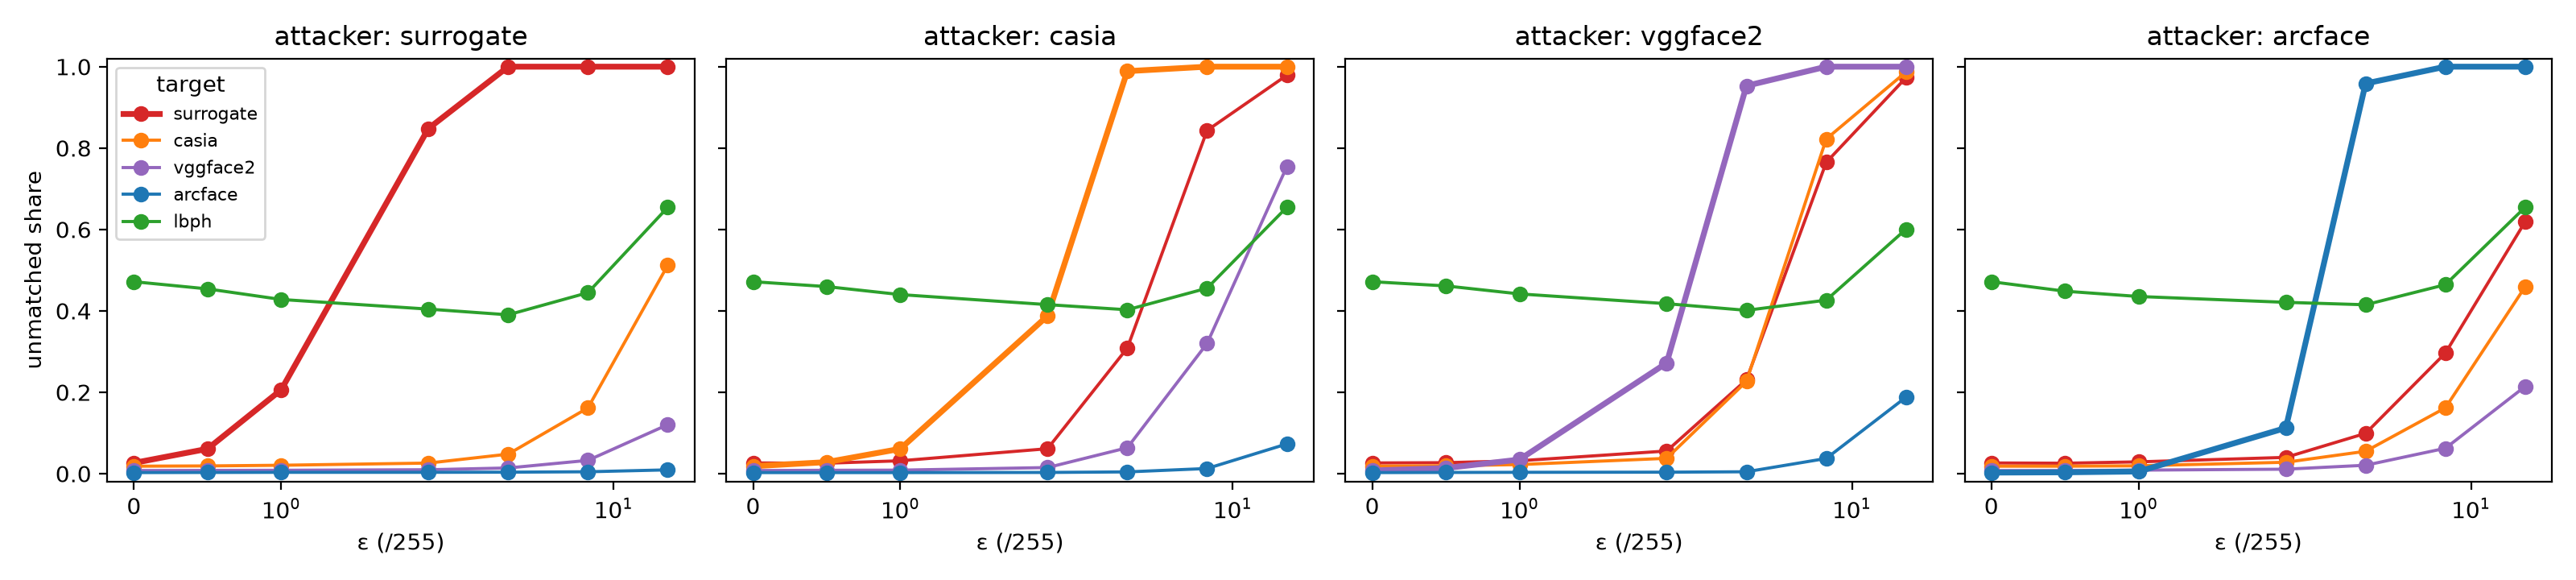
\includegraphics[width=17.4cm]{figures/attacker_transfer.png}
\caption{Unmatched share against $\varepsilon$ for each attacker (one panel each), one line per target model; the thick line is the attacker scored on itself.}
\end{figure}

\needspace{6\baselineskip}\subsection{What changes}

\textbf{Our surrogate is the weakest attacker.} At $\varepsilon$ = 8/255 its edits make casia lose 16.2\% and vggface2 3.3\%. Edits built against vggface2 make casia lose 82.2\%; edits built against casia make vggface2 lose 32.0\%. So the low transfer in Section 6 is partly a property of our surrogate, and ``edits barely transfer'' was too strong as a general statement.


\textbf{But it is not a broken model; it is an easy target.} Edits from casia and vggface2 make the surrogate lose 84.3\% and 76.5\% of pairs at $\varepsilon$ = 8/255, and 30.9\% and 23.1\% at $\varepsilon$ = 4/255. It is fragile, and its own gradients point in directions the other models do not share.


\textbf{Architecture matters more than training data.} The three InceptionResnetV1 models fool each other well even when their training faces differ: vggface2 $\to$ casia is 82.2\% at $\varepsilon$ = 8/255 and 98.7\% at 16/255. ArcFace, the only different architecture, resists every attacker: the best is vggface2 at 18.8\%, and only at a clearly visible $\varepsilon$ = 16/255. In the other direction, ArcFace's own edits reach the InceptionResnetV1 models only moderately (61.9\% surrogate, 45.9\% casia, 21.4\% vggface2 at $\varepsilon$ = 16/255).


\textbf{Transfer is lopsided.} vggface2 $\to$ casia (82.2\% at $\varepsilon$ = 8/255) is much stronger than casia $\to$ vggface2 (32.0\%). The model trained on the larger, more varied VGGFace2 data is both the strongest attacker and the hardest InceptionResnetV1 model to fool.


\textbf{Invisible edits still transfer only partially.} At $\varepsilon$ = 4/255 (SSIM about 0.96) the strongest transfer between any two different deep models is casia $\to$ surrogate at 30.9\%; at $\varepsilon$ = 2/255 nothing transfers above 6.1\%. JPEG after editing reduces transfer slightly (e.g. vggface2 $\to$ casia 82.2\% $\to$ 74.7\% at $\varepsilon$ = 8/255).


\textbf{LBPH} sits at 42.6\%--46.4\% at $\varepsilon$ = 8/255 whichever model built the edit, which supports treating it as noise-sensitive rather than fooled (Section 10).


\textbf{Why might our surrogate be a weak attacker?} These are untested hypotheses: (1) \emph{overfitting}: training accuracy reached 97.4\% while LFW accuracy plateaued, and we used the final epoch rather than the best; (2) \emph{crop geometry}: the surrogate aligns faces by landmarks, while casia and vggface2 use a box crop, so edits shaped through one geometry may carry over worse to the other (ArcFace, which also uses landmark alignment, transfers better to the surrogate, 29.6\%, than to casia, 16.2\%, at $\varepsilon$ = 8/255); (3) \emph{training budget}: 30 epochs on CASIA alone, much less than the pretrained models received.


\clearpage

\needspace{6\baselineskip}\subsection{What the edits look like}

To make the tables concrete, we picked 3 same-person pairs (one from each of three different folds, chosen at random among pairs that all four deep models match before editing): Vanessa Incontrada, Vanessa Williams, Doris Schroeder. For each pair we edited photo \emph{a} with PGD against each attacker at $\varepsilon$ = 0, 2, 4, 8 and 16/255, with exactly the sweep's settings (20 steps, random start, seed 0, rounded to 8-bit), and scored every edited photo on all five models with each model's fold threshold. GPU computation is not bit-for-bit reproducible even with a fixed seed, so re-running can flip a tag for a model sitting right at its threshold (3 of the 300 tags changed between two runs); the overall pattern does not change.


\textbf{How to read the grids.} Rows are attackers, columns are budgets; the first column is the photo \emph{b} the edited photo is compared against. Under each image are five tags, one per target model: \textbf{S} surrogate, \textbf{C} casia, \textbf{V} vggface2, \textbf{A} arcface, \textbf{L} lbph. A \textcolor{tagred}{\textbf{red}} tag means that model no longer matches the pair (the edit fooled it); grey means it still recognises the person. The SSIM between the edited and original photo is printed underneath. Images show the central 190$\times$190 pixels of the 250$\times$250 photo. Examples were chosen so that all four deep models match the pair before editing; LBPH, with its 67\% clean accuracy, already misses two of the three pairs, so its L tag is red even at $\varepsilon$ = 0.


\textbf{What they show.} The single photos follow the same pattern as the tables. In the first example, our surrogate's edit fools only the surrogate up to $\varepsilon$ = 8/255 (fooled: surrogate), while the vggface2 edit at the same budget fools surrogate, casia, vggface2 and the casia edit fools surrogate, casia, vggface2. ArcFace's edit fools only ArcFace until $\varepsilon$ = 16/255 (surrogate, casia, vggface2, arcface, lbph). At 2--4/255 the edits are hard to see; at 16/255 a grainy texture is clearly visible, especially on skin.


\begin{figure}[H]\centering
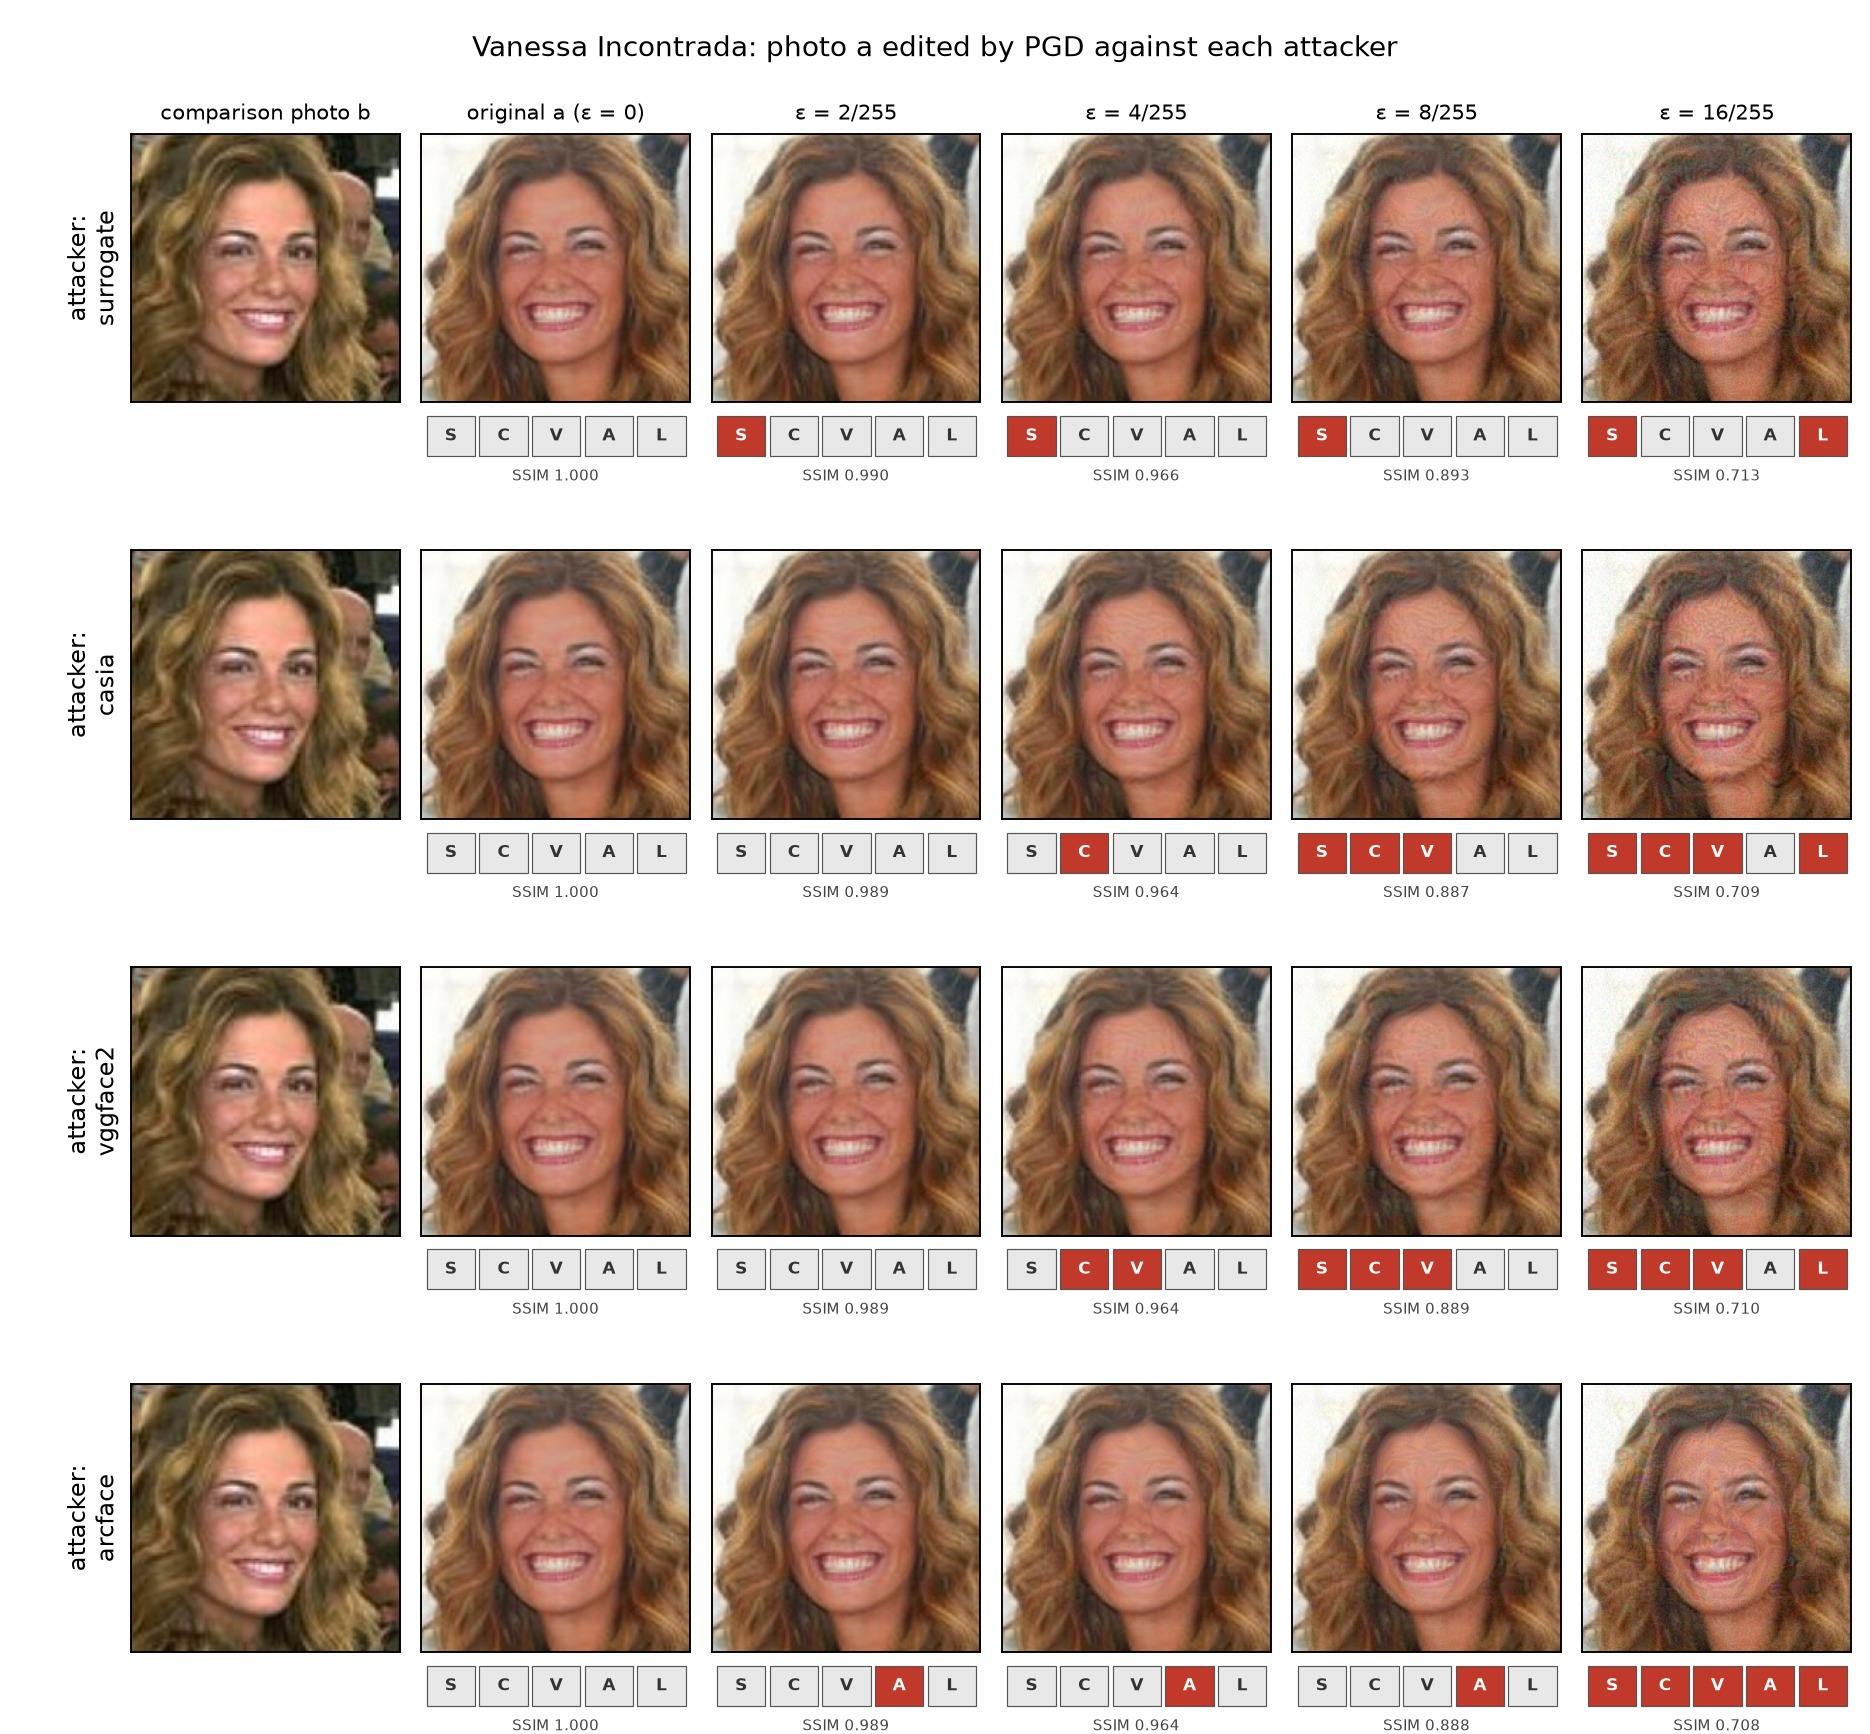
\includegraphics[width=16.0cm]{figures/example_0.jpg}
\caption{Vanessa Incontrada: photo a edited against each attacker (rows) at each budget (columns). Tags: models fooled (red) or still matching (grey); S surrogate, C casia, V vggface2, A arcface, L lbph.}
\end{figure}

\clearpage

\begin{figure}[H]\centering
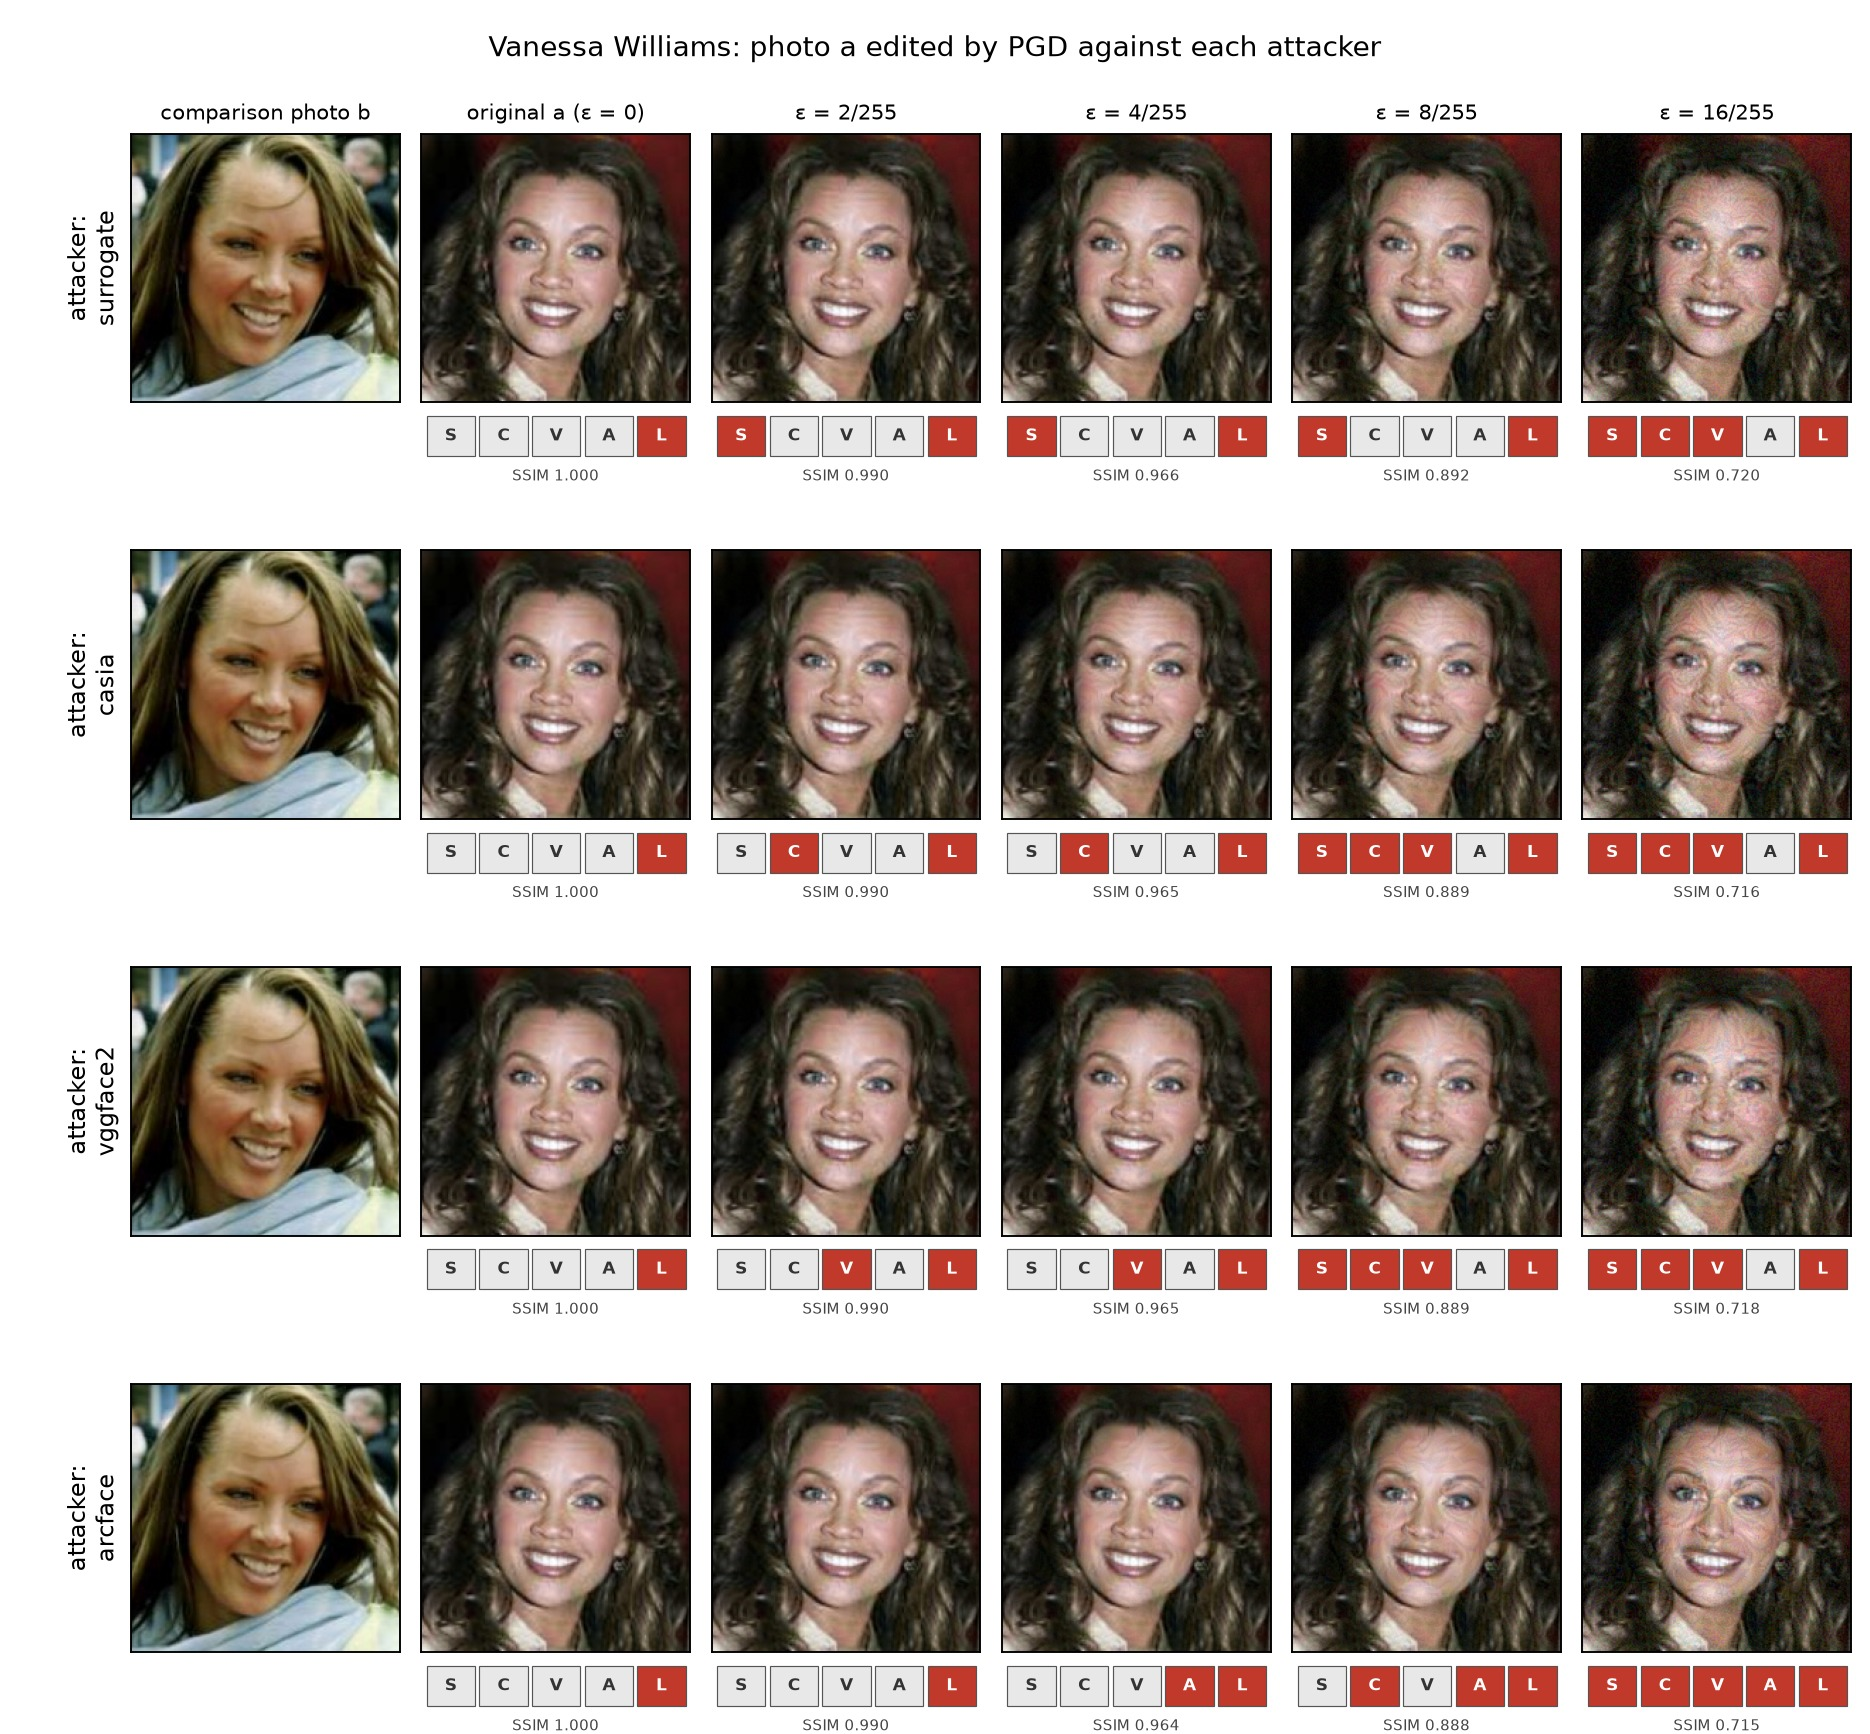
\includegraphics[width=17.4cm]{figures/example_1.jpg}
\caption{Vanessa Williams: photo a edited against each attacker (rows) at each budget (columns). Tags: models fooled (red) or still matching (grey); S surrogate, C casia, V vggface2, A arcface, L lbph.}
\end{figure}

\clearpage

\begin{figure}[H]\centering
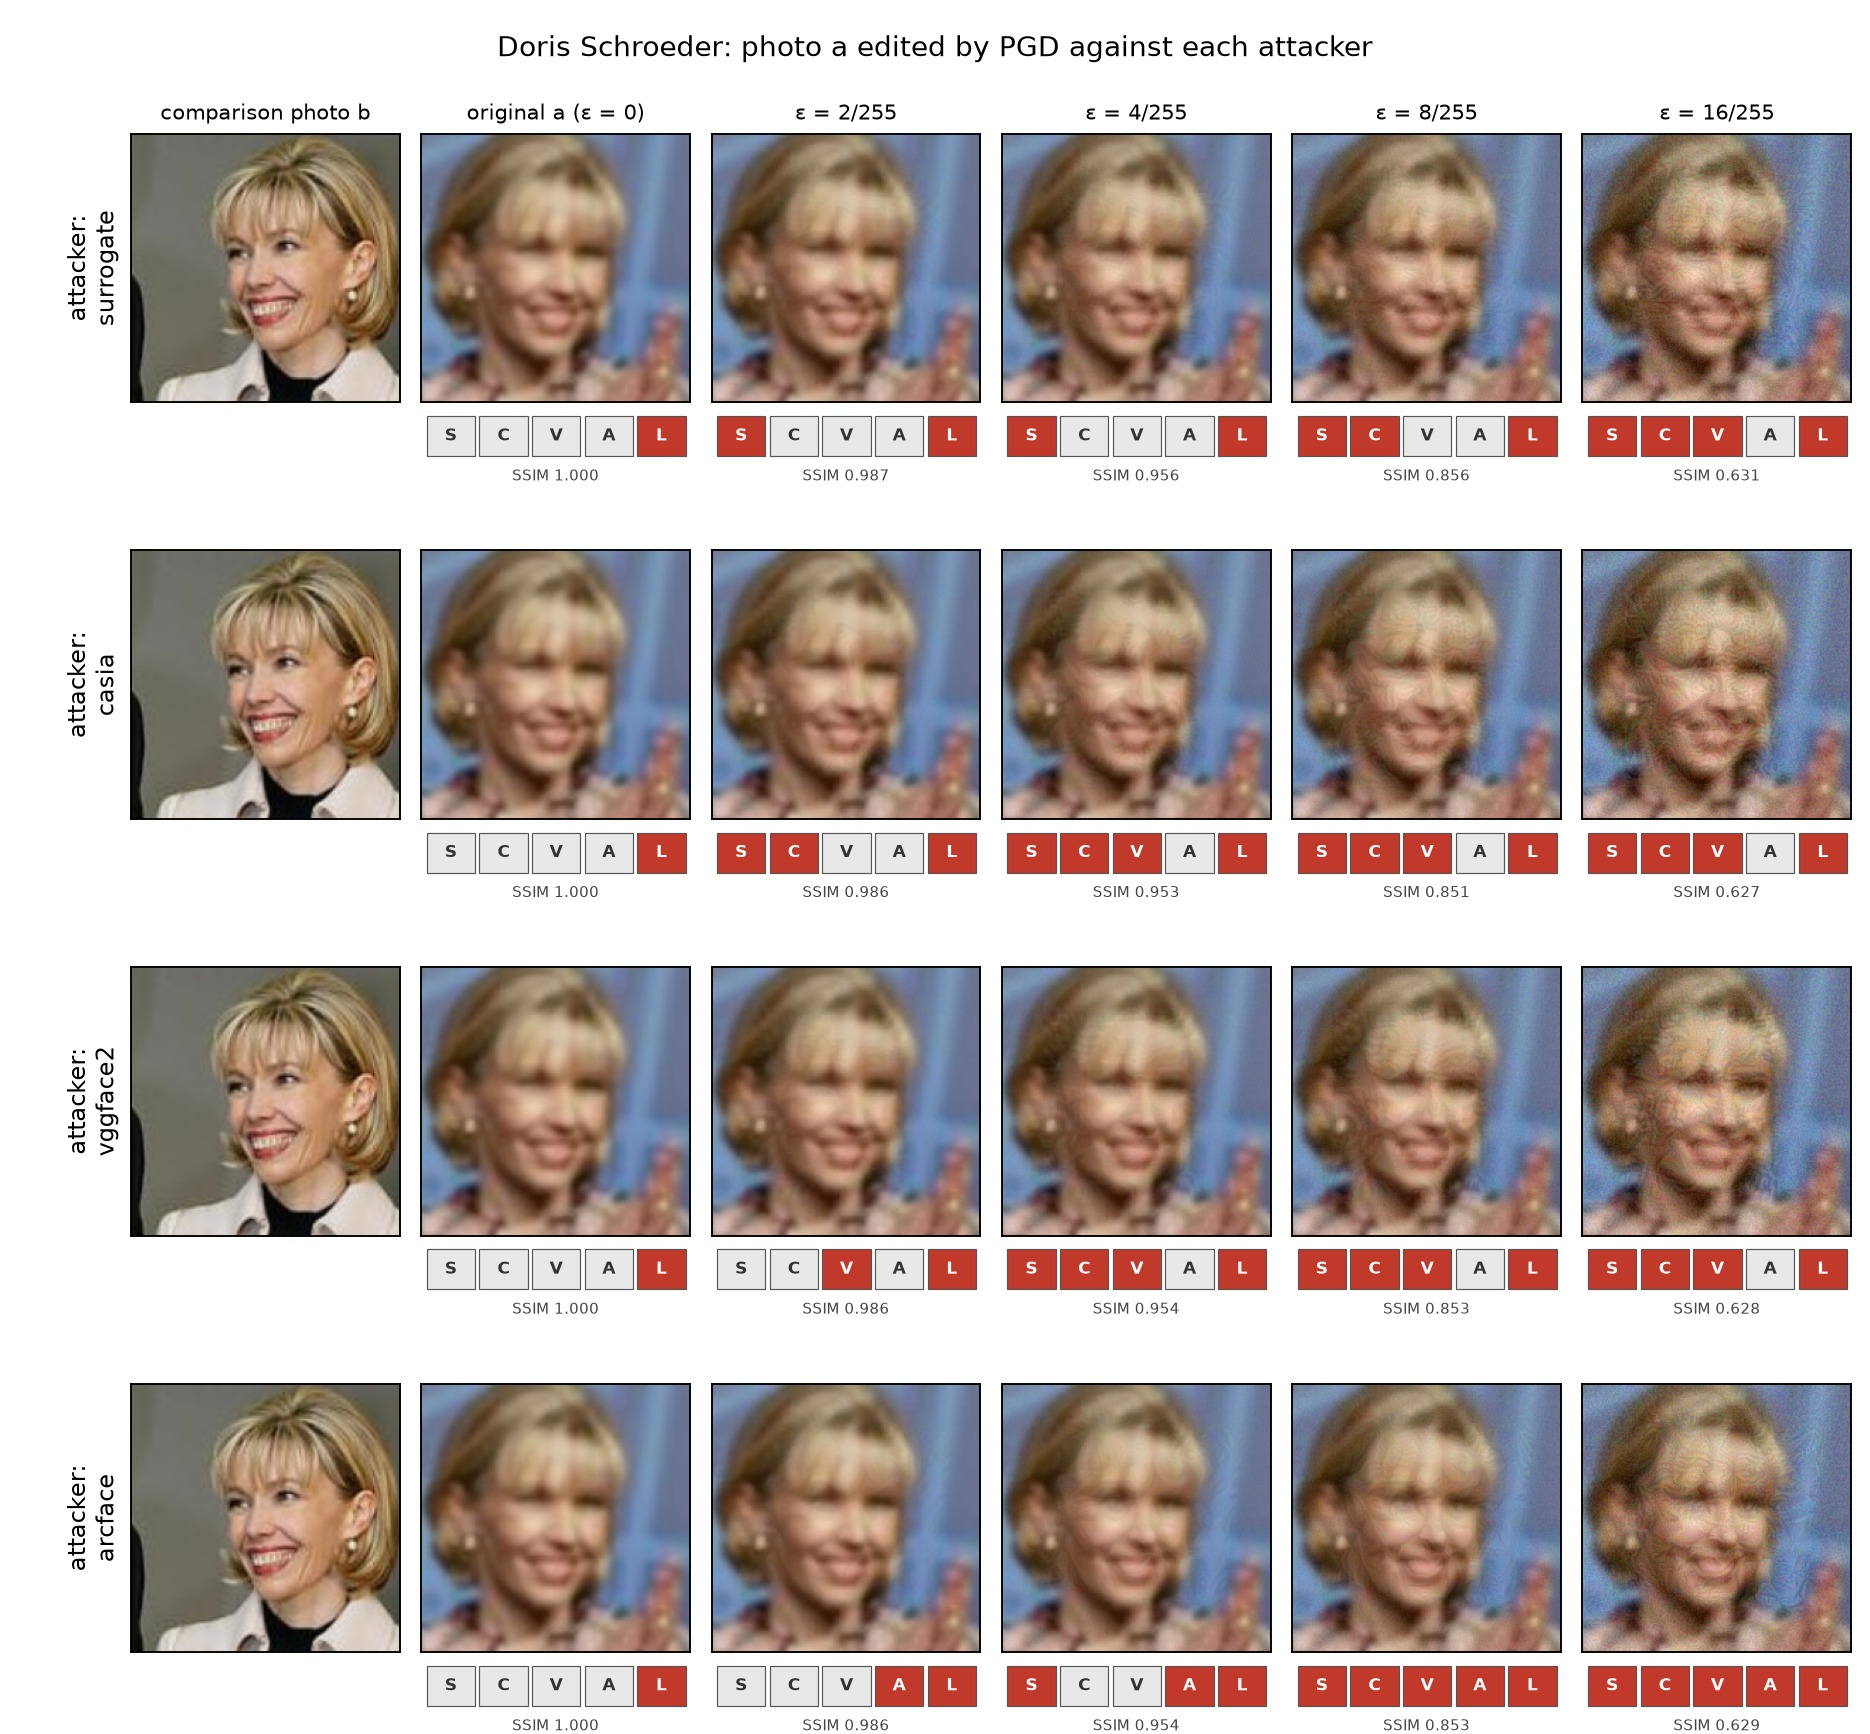
\includegraphics[width=17.4cm]{figures/example_2.jpg}
\caption{Doris Schroeder: photo a edited against each attacker (rows) at each budget (columns). Tags: models fooled (red) or still matching (grey); S surrogate, C casia, V vggface2, A arcface, L lbph.}
\end{figure}

\clearpage

\needspace{6\baselineskip}\subsection{The edits on their own}

The figure below shows only the change each attacker made to the first example (edited minus original), with each column scaled by 1/$\varepsilon$ so the pattern is visible at every budget (mid-grey = no change). Three things stand out:


\begin{itemize}
  \item  \textbf{The pretrained attackers' edits are face-shaped.} The casia, vggface2 and arcface edits trace the eyes, brows, mouth and outline of the face, so they change the facial features a recognition model relies on. Our surrogate's edit looks like unstructured texture with little facial structure. This is a plausible visual explanation for why its edits transfer so poorly (Section 9.1), though we have not tested it formally.
  \item  \textbf{Each edit stays inside its attacker's crop.} PGD can only change pixels the attacker actually looks at, so each edit is a rectangle matching that model's crop: a landmark-aligned square for the surrogate and arcface, the MTCNN box with margin for casia and vggface2. An edit built through one crop may miss part of another model's crop.
  \item  \textbf{The rest is PGD's random start.} Outside the crop, the speckle is the random starting noise, which no gradient ever updates. It is the same for every attacker and slightly lowers SSIM; it is not part of the optimised edit.
\end{itemize}

\begin{figure}[H]\centering
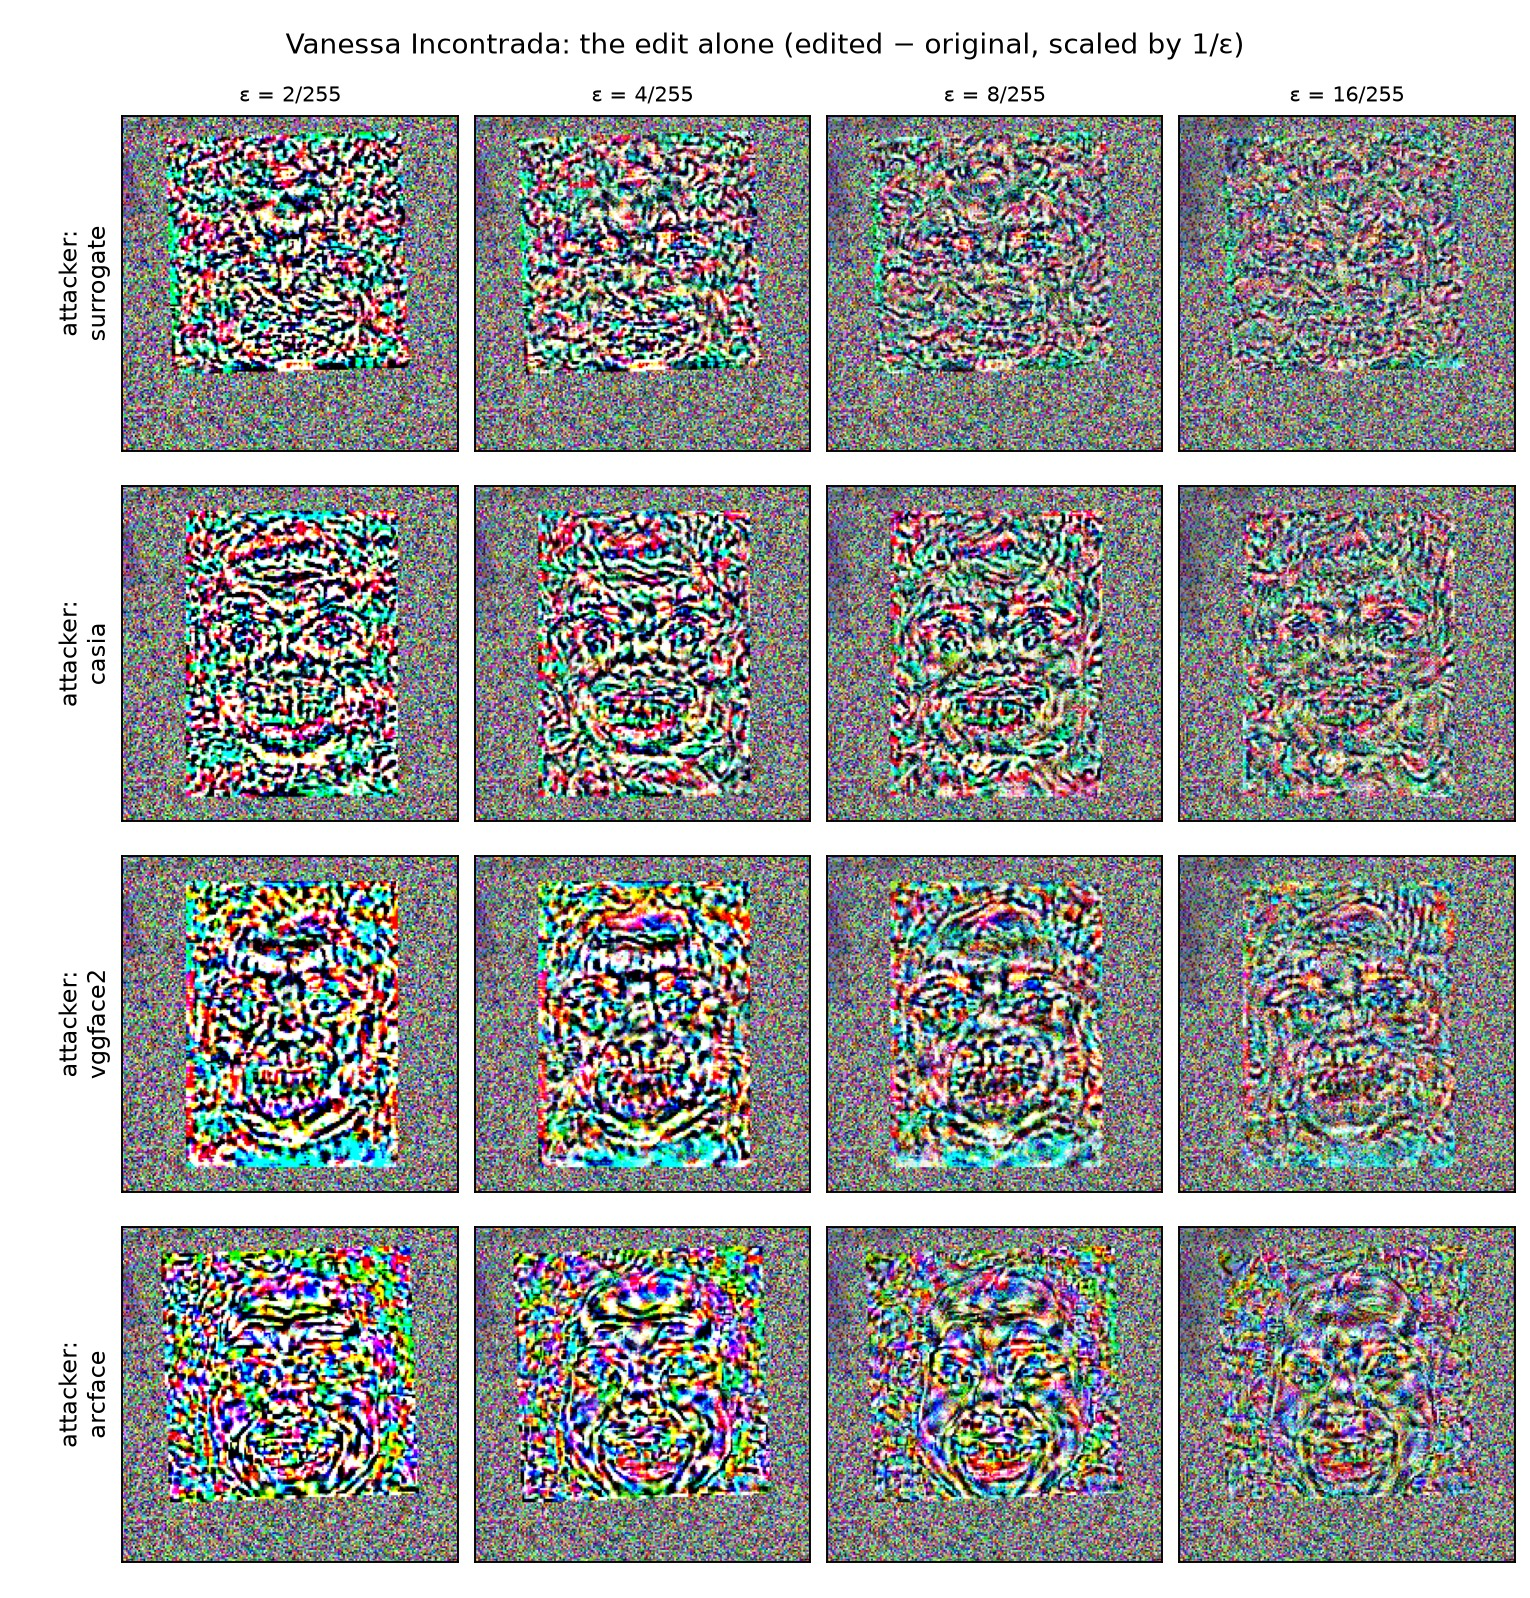
\includegraphics[width=14.5cm]{figures/perturbation_0.jpg}
\caption{Vanessa Incontrada: the edit alone (edited $-$ original) for each attacker and budget, each column scaled by 1/$\varepsilon$. Edits for the other two examples are in runs/examples/.}
\end{figure}

\needspace{8\baselineskip}\section{A note on LBPH (the non-deep model)}

LBPH needs careful interpretation. Its clean accuracy is only 67.0\%, so with its best threshold it already fails to match 47.2\% of same-person pairs before any edit. Its numbers also move in the opposite direction from what transfer would predict: small PGD edits slightly \emph{lower} its unmatched share (47.2\% $\to$ 39.0\% at $\varepsilon$ = 4/255), random noise affects it far more than PGD at $\varepsilon$ = 16/255 (90.1\% vs 65.4\%), and blur at $\sigma$ = 3 breaks it almost completely (99.6\%).


LBPH describes faces by fine local texture, so any change to pixel-level texture moves its distances, whether or not the change is targeted. Its numbers therefore measure sensitivity to pixel changes in general, not transfer of the edit, and it should be reported as a non-deep baseline rather than as evidence that the edit transfers.


\needspace{8\baselineskip}\section{Conclusions}

1. \textbf{Edits built against our surrogate transfer poorly.} A nearly invisible edit ($\varepsilon$ = 4/255) that fully defeats the surrogate leaves every other deep model recognising about 95\% or more of the same-person pairs.


2. \textbf{The results are stable.} Across three random seeds no result's standard deviation exceeds 0.69 percentage points.


3. \textbf{Transfer depends strongly on which model the edit is built against.} Our surrogate is the weakest of four attackers: edits built against vggface2 make casia lose 82.2\% of pairs at $\varepsilon$ = 8/255, against 16.2\% for our surrogate.


4. \textbf{Architecture matters more than training data.} Models sharing the InceptionResnetV1 architecture fool each other well even with different training faces, while ArcFace resists every attacker (at most 18.8\%, and only at a visible $\varepsilon$ = 16/255). The surrogate-only result that seemed to favour training data (Section 6) does not generalise.


5. \textbf{The effect comes from the optimisation.} Random noise of the same size, JPEG compression and mild blur do almost nothing to the deep models.


6. \textbf{Implication for privacy tools.} Protection built against one recognition system is unreliable against an unknown one: it depends on the tool's choice of model, it is much weaker against a different architecture, and at a nearly invisible budget ($\varepsilon$ = 4/255) even the best pairing transfers to only 30.9\% of pairs.


\needspace{8\baselineskip}\section{Limitations and next steps}

\begin{itemize}
  \item  One editing method (PGD) and one budget sweep. Attacking an ensemble of models at once, the standard way to make edits transfer better, was not tried.
  \item  Seeds 1 and 2 were run with the surrogate as attacker only; the other attackers use seed 0. Seed spread for the surrogate is under 0.7 points, so this is unlikely to matter.
  \item  The saved surrogate is the final epoch (98.12\% clean LFW), not the best epoch (98.32\%). Why it is a weak attacker (overfitting, crop geometry, training budget) is untested; keeping the best checkpoint, or retraining with a box crop, would test two of those.
  \item  The original seed-0 sweep scored ArcFace with onnxruntime; all later runs use the PyTorch conversion. Both give identical clean accuracy, and ArcFace's numbers agree across the three seeds to within 0.13 points.
  \item  Face landmarks come from the clean photo and are reused for its edited versions; a real system would re-detect the face, which large edits could shift.
  \item  The proposal's optional check of whether protection holds equally across demographic groups (LFW is roughly 77.5\% male and 83.5\% White) has not been done yet.
  \item  LBPH's low clean accuracy limits what its numbers can show (Section 10).
  \item  PGD's random start adds noise to the whole photo, but only pixels inside the attacker's crop are then optimised, so the noise outside the crop stays (Section 9.3). It slightly lowers SSIM equally for every attacker; starting from the clean photo, or masking the start to the crop, would remove it.
\end{itemize}

{\small\color{subtle} An early smoke test on a random subset of 200 pairs ($\varepsilon$ = 0, 4, 16) gave the same pattern as the full run, e.g. casia 56.3\% and arcface 1.8\% at $\varepsilon$ = 16/255. All figures in this document use the full 3,000-pair run.\par}

\end{document}
